
% -----------------------------------------------------


% Document and Formatting

\documentclass[a4paper, 11pt, dvipsnames]{scrartcl}

\usepackage[margin=2cm, bottom=3cm]{geometry}
\usepackage[colorlinks = true, allcolors = black, urlcolor = Mahogany]{hyperref}
\usepackage{charter}
\usepackage{setspace}
\usepackage[english]{babel}
\usepackage[charter]{mathdesign}
\usepackage[gen]{eurosym}
\usepackage{csquotes}
\usepackage{soul}

\setstretch{1.1}
\addtokomafont{disposition}{\rmfamily}
\addtokomafont{section}{\rmfamily}
\addtokomafont{subsection}{\rmfamily}
\addtokomafont{subsubsection}{\rmfamily}
\addtokomafont{title}{\rmfamily}
\addtokomafont{subtitle}{\rmfamily}
\setlength{\parskip}{0.5em}
\setlength{\parindent}{0em}
\MakeOuterQuote{"}
%\let\mathcal\undefined
%\DeclareMathAlphabet{\mathcal}{OMS}{cmsy}{m}{n}
\setul{2pt}{0.5pt}


% Section Titles

\newcommand{\myrule}{\begin{center} \vspace{-24pt} \color{Mahogany} \rule{\textwidth}{1pt} \end{center}}
\newcommand{\tmpsection}[1]{}
\let\tmpsection=\section
\renewcommand{\section}[1]{\tmpsection{#1}\vspace{-0.25em}\myrule\vspace{-2em}}

\newcommand{\tmpsubsection}[1]{}
\let\tmpsubsection=\subsection
\renewcommand{\subsection}[1]{\tmpsubsection{#1}\vspace{-0.5em}}

\newcommand{\tmpsubsubsection}[1]{}
\let\tmpsubsubsection=\subsubsection
\renewcommand{\subsubsection}[1]{\tmpsubsubsection{#1}\vspace{-0.5em}}


% Boxes

\usepackage{tcolorbox}

\newtcolorbox{mybox}{colback=Orange!20!white,arc=12pt,boxrule=0pt, halign=flush center, colframe=white}


% Math

%\usepackage{amsmath}
%\usepackage{amssymb}
\newcommand\hmmax{0}
\newcommand\bmmax{0}
\usepackage{bm}
\usepackage{array}
\usepackage{mathtools}
\usepackage{cancel}

\newcommand{\qed}{\hfill\blacksquare}
\newcommand{\qedwhite}{\hfill \ensuremath{\Box}}
\newcommand{\ind}{\perp\!\!\!\!\perp} 


% Special Environments

\usepackage{booktabs}
\usepackage{enumitem}
\usepackage{graphicx}
\usepackage{tikz}
\usepackage{pgfplots}
\usepackage{float}

\setlist[enumerate,1]{label={(\arabic*)}}


% Headers and Footers

\usepackage{fancyhdr}
\usepackage{lastpage}

\pagestyle{fancy}
\fancyhead{}\renewcommand{\headrulewidth}{0pt}
\fancyfoot{}\renewcommand{\footrulewidth}{0.5pt}
\fancyfoot[L]{\zfauthor}
\fancyfoot[C]{\thepage/\color{black}\pageref{LastPage}\\
\hyperlink{toc}{\color{gray}\scriptsize{Go to table of contents}}}
\fancyfoot[R]{\zfdate}


% Table of Contents

\usepackage{tocloft}

\renewcommand{\cftsecleader}{\cftdotfill{\cftdotsep}}
\cftpagenumbersoff{subsection}
\setcounter{tocdepth}{2}
\setcounter{secnumdepth}{1}
\setcounter{section}{0}


% Numbering

\numberwithin{equation}{section}
\numberwithin{figure}{section}
\numberwithin{table}{section}


% Miscellaneous

\usepackage{lipsum}


% Watermarks

%\usepackage{draftwatermark}
%\SetWatermarkText{\textbf{PRELIMINARY}}
%\SetWatermarkScale{0.55}


% Boxes

\usepackage{tcolorbox}

\tcbuselibrary{skins,breakable}

\newtcolorbox[auto counter, number within=section, number freestyle={\noexpand\thesection.\noexpand\arabic{\tcbcounter}}]{proofbox}[2][]{%
    enhanced,
    breakable,
    colback=MidnightBlue!10,
    colframe=MidnightBlue,
    colupper=MidnightBlue!50!black,
    fonttitle=\bfseries,
    title=Proof: #2,
    #1
}

\newtcolorbox[auto counter, number within=section, number freestyle={\noexpand\thesection.\noexpand\arabic{\tcbcounter}}]{defbox}[2][]{%
    enhanced,
    breakable,
    colback=Maroon!10,
    colframe=Maroon,
    fonttitle=\bfseries,
    title=#2,
    #1
}

\newtcolorbox[auto counter, number within=section, number freestyle={\noexpand\thesection.\noexpand\arabic{\tcbcounter}}]{exbox}[2][]{%
    enhanced,
    breakable,
    colback=Orange!10,
    colframe=Orange,
    fonttitle=\bfseries,
    title=Example: #2,
    #1
}




\newcommand{\Var}[1]{\ensuremath{\mathrm{Var}\left({#1}\right)}}
\newcommand{\E}[1]{\ensuremath{\mathrm{E}\left({#1}\right)}}
\newcommand{\Cov}[1]{\ensuremath{\mathrm{Cov}\left({#1}\right)}}
\newcommand{\Cor}[1]{\ensuremath{\mathrm{Cor}\left({#1}\right)}}


\newcommand{\zftitle}{Advanced Macroeconometrics}
\newcommand{\zfauthor}{Max Heinze}
\newcommand{\zfdate}{Summer Term 2023}

\begin{document}


\hypertarget{toc}{}

{
\color{gray}
\hrule height 1pt
}

\vspace{0.25em}

{
\LARGE
\color{Mahogany}
\textbf{\zftitle} \par
}

\vspace{-0.5em}

{
\large
\color{gray}
\textbf{\zfauthor, \zfdate} \par
}

\vspace{0.75em}

{
\color{gray}
\hrule height 1pt
}

\tableofcontents
\thispagestyle{fancy}

\pagebreak

\setcounter{section}{-1}


% -----------------------------------------------------

\section{Preliminaries}

\subsection{Statistics}

\subsubsection{Expectation, Variance, Moments}

Informally, the \textbf{expected value} of a \textbf{random variable} is the mean of a large number of independent draws of that variable, or in short, the \textbf{mean} of the random variable. We can think of the expected value of a \textbf{distribution} as a measure of the distribution's center. 

The $n$-th \textbf{central moment} is defined as $\mu_n=\mathrm{E}(X-\mu)^n$. Thus, the variance, the second central moment, equals $\mathrm{Var}(X) = \mathrm{E}((X-\mu)^2) = \mathrm{E}(X^2) - \mathrm{E}(X)^2$.

For constants $a, b,c \in \mathbb{R}$ functions $g(\cdot)$ and $h(\cdot)$ as well as random variables $X$ and $Y$,

\begin{align}
	\mathrm{E}(ag(X)+bh(Y)+c) &= a\mathrm{E}(g(X)) + b\mathrm{E}(h(Y)) + c \\
	\mathrm{E}(XY) &\neq \mathrm{E}(X)\mathrm{E}(Y) \qquad\text{\textbf{except} if $X$ and $Y$ are independent} \\
	\mathrm{Var}(ag(X)+bh(Y)+c) &= a^2\:\mathrm{Var}(g(X)) + b^2\:\mathrm{Var}(h(Y)) + 2ab\:\mathrm{Cov}(g(x), h(Y)) \\
	\mathrm{Cov}(X,Y) &= \mathrm{E}\big((X-\mathrm{E}(X))\:\:(Y-\mathrm{E}(Y))\big) = \mathrm{E}(XY) - \mathrm{E}(X)\mathrm{E}(Y)
\end{align}

\subsubsection{Notation}

We can denote a time series as a \textbf{stochastic process}:

\[
	\{y_t:t=1,2,\dots,T\}.
\]

To denote earlier values, we can use the \textbf{lag operator}:

\[
	\mathrm{L}y_t = y_{t-1}, \quad\mathrm{L}^2y_t = y_{t-2}. 
\]

To denote differences, we can use the \textbf{difference operator}:

\[
	\Delta y_t = y_t-y_{t-1}.
\]

\subsubsection{Variance-Covariance Matrix}

Consider a univariate time series. Its variance is given by

\begin{equation}
	\Var{\{y_t\}_{t=1}^T} = \sum^T_{t=0}\frac{(y_t-\bar{y})^2}{N} = \sum^T_{t=0}\frac{(y_t-\bar{y})(y_t-\bar{y})}{N}.
\end{equation}

If $\bm{y}_t$ is a vector of $M$ time series, the formula yields a variance-covariance matrix of the following form:

\begin{equation}
	\begin{bmatrix}
		\Var{y_{1t}} & \Cov{y_{1t},y_{2t}} & \dots & \Cov{y_{1t},y_{Mt}} \\
		\Cov{y_{2t},y_{1t}} & \Var{y_{1t}} & \dots & \Cov{y_{2t},y_{Mt}} \\
		\vdots & \vdots & \ddots & \vdots \\
		\Cov{y_{Mt},y_{1t}} & \Cov{y_{Mt},y_{2t}} & \dots & \Var{y_{Mt}}
	\end{bmatrix}
\end{equation}

\subsection{Table of Probability Distributions}

\begin{tabular}{|l|c|c|c|c|c|}
	\hline
	\multicolumn{6}{|l|}{\textbf{Discrete Distributions}} \\ \hline
	\textbf{Distribution} & \scalebox{0.8}[1]{\textbf{Parameters}} & \textbf{Mean} & \textbf{Variance} & \textbf{Probability Mass Function} & \textbf{Conjugate Prior}	\\ \hline
	\textit{Bernoulli} & $p$ & $p$ & $p(1-p)$ & $f(k\mid p) = p^k(1-p)^{n-k}$ & Beta \\ \hline
	\textit{Binomial} & $n,p$ & $np$ & $np(1-p)$ & $f(k\mid n, p) = \binom{n}{k}p^k(1-p)^{n-k}$ & Beta \\ \hline
	\textit{Poisson} & $\lambda$ & $\lambda$ & $\lambda$ & $f(k\mid \lambda) = \frac{\lambda^ke^{-\lambda}}{k!}$ & Gamma \\ \hline
	\multicolumn{6}{|l|}{\textbf{Continuous Distributions}} \\ \hline
	\textbf{Distribution} & \scalebox{0.8}[1]{\textbf{Parameters}} & \textbf{Mean} & \textbf{Variance} & \textbf{Probability Density Function} & \textbf{Conjugate Prior}	\\ \hline
	\textit{Normal} & $\mu, \sigma^2$ & $\mu$ & $\sigma^2$ & \scalebox{0.7}[0.9]{$f(\theta\mid \mu,\sigma) = (2\pi\sigma^2)^{-\frac{1}{2}}\mathrm{exp}\left(-\frac{1}{2\sigma^2}(\theta-\mu)^2\right)$} & \begin{tabular}{lr}$\mu$: & N \\ $\sigma^2$: & G${}^{-1}$ \\ $\mu,\sigma^2$: & ---\end{tabular} \\ \hline
	\textit{Beta} & $\alpha,\beta$ & $\frac{\alpha}{\alpha+\beta}$ & \scalebox{0.7}[0.9]{$\frac{\alpha\beta}{(\alpha+\beta)^2(\alpha+\beta+1)}$} & $f(\theta\mid \alpha,\beta) = \frac{\theta^{\alpha-1}(1-\theta)^{\beta-1}}{\mathrm{B}(\alpha,\beta)}$ &  \\ \hline
	\textit{Gamma} & $\alpha, \beta$ & $\frac{\alpha}{\beta}$ & $\frac{\alpha}{\beta^2}$ & $f(\theta\mid \alpha,\beta) = \frac{\theta^{\alpha-1}e^{-\beta \theta}\beta^{\alpha}}{\Gamma(\alpha)}$ & Gamma \\ \hline
	\textit{Inverted Gamma} & $\alpha, \beta$ & $\frac{\beta}{\alpha-1}$ & $\frac{\beta^2}{(\alpha-1)^2(\alpha-2)}$ & \scalebox{0.8}[0.9]{$f(\theta\mid\alpha,\beta) = \frac{\beta^\alpha}{\Gamma(\alpha)}\theta^{-\alpha-1}\mathrm{exp}\left(-\frac{\beta}{\theta}\right)$} & Gamma \\ \hline
	\textit{Multivar. Normal} & $\bm{\mu}, \bm{\Sigma}$ &  &  &  & {N.--Inv. Wishart} \\ \hline
\end{tabular}


% -----------------------------------------------------

\section{Univariate Time Series}

\subsection{Time Series Data}

\subsubsection{Characteristics of Time Series}

Time series are observations of quantities that carry a time index:

\[
	x_t.
\]

Unlike in cross-sectional analysis, where we treat observations of individuals, $x_i$, this index carries meaning and indices are not arbitrarily interchangable. We cannot simply assume that observations are independent, they are usually dependent on prior realizations of themselves. 

In economics, we often encounter time series data that is measured at annual, quarterly, or monthly frequency. Examples for this include GDP, the unemployment rate, inflation, and many more. We can analyze this data with different purposes in mind, namely, description, causal inference, and prediction.

Consider the following time series: 

\begin{align}
	\{y_t&:t=1,\dots, T\}, \\
	\nonumber \{x_t&:t=1,\dots, T\}, \\
	\nonumber \{\varepsilon_t&:t=1,\dots, T\}, \quad \varepsilon_t\sim\mathcal{N}(0,\sigma^2).
\end{align}

Imagine we applied standard linear OLS methods and estimated

\[
	y_t = x_t\beta + \varepsilon_t, \quad \varepsilon_t \sim \mathcal{N}(0,\sigma^2),
\]

applying the assumptions that $\mathrm{E}(\varepsilon_t)=0$, $\mathrm{Var}(\varepsilon_t)=\sigma^2$, and $\mathrm{Cov}(\varepsilon_t,\varepsilon_s)=0 \quad\forall t\neq s$. The third assumption, assuming independence of individual realizations of the error, would be unreasonable in time series contexts, since adjacent values of the error term are often correlated.

Using regular OLS methods to regress one time series on another will very often lead to the coefficient $\beta_j$ being significantly different from zero, no matter whether there is a relation or not. This is referred to as the \textbf{spurious regression problem}.

Instead of using the model 

\[
	y_i = \beta_0 + x_{i1}\beta_1 + x_{i2}\beta_2 + \dots + x_{iK}\beta_K + \varepsilon_i,
\]

where we can answer questions about ceteris paribus effects and rely on exogeneity of $x_{ij}$, i.e. $\mathrm{E}(\varepsilon_i\mid x_{i1},\dots,x_{iK}) = 0$, we can use the model

\begin{equation}
	y_t = \beta_0 + \delta y_{t-1} + x_{t1}\beta_1 + x_{t2}\beta_2 + \dots + x_{tK}\beta_K + \varepsilon_t,
\end{equation}

where we explicitly model the development of the time series as well. Note that a change in one of the $x_{ij}$ not only has an effect on $y_t$, but also on all other subsequent realizations of $y$.

\subsubsection{Components of Time Series}

For a given time series, variation can come from different sources:

\begin{equation}
	y_t = \mu_t + c_t + \varepsilon_t,
\end{equation}

where $\mu_t$ is a \textbf{trend} component, $c_t$ is a \textbf{cyclical} component, and $\varepsilon_t$ is an \textbf{irregular} component. The trend component covers long term changes in the mean of the time series over time, the cyclical component covers seasonal (e.g., weekday effects) and non-seasonal (e.g., business cycles) oscillations, and the irregular component covers random fluctuations when all other components have been removed.

Usually, we are interested in the random part of the time series. For analyzing this, we have to remove the fixed parts, i.e., \textbf{detrend} the time series. We can do this a number of ways, such as:

\begin{enumerate}[label = (\arabic*)]
	\item Using \textbf{growth rates} such as year-on-year or month-on-month growth.
	\item Linear or non-linear \textbf{de-trending}, deterministic \textbf{de-seasonalizing},
	\item Applying a \textbf{filter} (such as the Bandpass Filter or the Hodrick-Prescott Filter).
\end{enumerate}

\subsection{Time Series Concepts and Properties}

\subsubsection{Autocovariance and Autocorrelation}

The \textbf{autocovariance function} at lag $j$ is given by

\begin{equation}
	\gamma(j) = \Cov{y_t,y_{t-j}} = \E{(y_t-\mu_t)(y_{t-j}-\mu_{t-j})},
\end{equation}

that is, the covariance of a value $y_t$ and the value $y_{t-j}$ $j$ periods before it. 

The \textbf{autocorrelation function} (ACF) at lag $j$ is then given by 

\begin{equation}
  \rho(j) = \Cor{y_t,y_{t-j}} = \frac{\Cov{y_t,y_{t-j}}}{\sigma^2} = \E{\frac{(y_t-\mu_t)(y_{t-j}-\mu_{t-j})}{\sigma^2}}.
\end{equation}

Both the autocovariance and the autocorrelation function provide information about the memory of the process, that is, how much information from past observation persists through to the current observation at time $t$. The values of the autocorrelation function can, like any correlation, never have an absolute value greater than 1:

\[
	-1 \leq \rho(j) \leq 1.
\]

In addition, by definition, $\rho(0)=1$. 

When dealing with real data, we can assess a time series's \textbf{empirical autocorrelation} given by

\begin{equation}
  \hat{\rho}(j) = \frac{1}{T} \sum^T_{t=j+1}\frac{y_t-\bar{y}_t}{s_y}\frac{y_{t-j}-\bar{y}
  _t}{s_y},
\end{equation}

where $s_y$ is the standard deviation of $y_t$. We often use plots of the empirical autocorrelation in order to assess the adjacency of time series value for different time series. It can also be used to assess the residuals of a regression.

\subsubsection{Durbin-Watson Test}

We can use the Durbin-Watson test to check whether first-order serial correlation of OLS residuals is present. The test statistic is given by:

\begin{equation}
  d = \frac{\sum^T_{t=2}(\hat{\varepsilon}_t-\hat{\varepsilon}_{t-1})^2}{\sum^T_{t=1}\hat{\varepsilon}^2_t}.
\end{equation}

In the case of no serial correlation, the expected value of the test statistic is $\E{d} = \frac{\E{\varepsilon_t^2}+\E{\varepsilon_{t-1}^2}}{\E{\varepsilon_t^2}} = \frac{2\sigma^2}{\sigma^2} = 2$. If the value of the test statistic is $0 \leq d < 2$, autocorrelation at lag 1 is positive, if the value of the test statistic is $2 < d \leq 4$, there is negative autocorrelation at lag 1. 

\subsection{Time Series Econometrics}

A \textbf{stochastic process} is a collection of random variables defined on a common probability space. A \textbf{time series} $\{y_t:t=1,\dots,T\}$ is a realization of a stochastic process in the time dimension. 

We observe the data, a time series, and try to infer the data-generating process, that is, the specific stochastic process that the time series is a realization of. The unconditional mean of the time series is $\E{y_t} = \mu$ and its variance is $\Var{y_t} = \sigma^2$. In general, the random variables $Y_t$ and $Y_s$ at different time points $t$ and $s$ are not independent of each other.

\subsubsection{Stationarity}

\textbf{Stationarity} is one important property of stochastic processes. Note that stationarity is a property of the stochastic process, and not of the time series, which is a realization of that process.

A stochastic process $\{y_t:t,1,\dots,T\}$ is said to be \textbf{covariance stationary} or \textbf{weakly stationary} if it fulfills the following three conditions:

\begin{enumerate}
	\item The \textbf{mean} is constant for all $t$:
	
	\[
		\E{y_t} = \mu \quad \forall t
	\]
	\item The \textbf{variance} is constant for all $t$:
	
	\[
		\Var{y_t} = \sigma^2 \quad \forall t
	\]
	\item The \textbf{covariance } at two time periods depends only on the difference between the two time periods, that is, the lag, and not on the actual time at which the covariance is computed. In other words, the autocorrelation is time invariant:
	\[
		\E{(y_t - \mu)(y_{t-j} - \mu)} = \gamma_j \quad \forall t \text{ and for any } j.
	\]
\end{enumerate}

A stochastic process $\{y_t:t,1,\dots,T\}$ is said to be \textbf{strictly stationary} if the joint distribution of $(y_{t1},y_{t2},\dots,y_{tk})$ is the same as that of $(y_{t1+h},y_{t2+h},\dots,y_{tk+h})$. That is, the joint distribution depends only on the difference $h$, not on time $t$. 

Weak stationarity does not imply strict stationarity, since it only requires the first two unconditional moments to be time invariant, while strict stationarity requires the whole joint distribution to be independent of time. Even the converse does not necessarily hold: Strict stationarity does not necessarily imply weak stationarity. However, it does imply weak stationarity when the first two unconditional moments exist and are finite. If the mean or variance do not exist or are not finite, then the process can be strictly stationary without being weakly stationary.

A process is called \textbf{trend stationary} if removing an underlying trend from the process results in a weakly stationary process. 

\subsection{Stationary Models}

\subsubsection{White Noise Process}

A white noise process is described by

\begin{equation}
  y_t = \varepsilon_t, \qquad \varepsilon_t \sim \mathcal{N}(0,\sigma^2).
\end{equation}

It is thus a sequence of random numbers. It is not autocorrelated beyond lag $j=0$. Any white noise process is weakly stationary. A white noise process as defined above is also strictly stationary.

\subsubsection{Moving Average Process}

A moving average (1), or MA(1) in short, process is defined as

\begin{equation}
  y_t = \mu + \varepsilon_t + \theta\varepsilon_{t-1}.
\end{equation}

Thus, $y_t$ is described as the weighted sum of the current error and past errors. If the coefficient $\theta = 0$, the process is reduced to a white noise process. 

The unconditional moments of an MA(1) process are

\begin{align*}
	\E{y_t} &= \mu, \\
	\gamma_0 &= \E{(y_t-\mu)^2} = (1+\theta^2)\sigma^2, \\
	\gamma_1 &= \E{(y_t-\mu)(y_{t-1}-\mu)} = \theta\sigma^2, \\
	\gamma_j &= \E{(y_t-\mu)(y_{t-j}-\mu)} = 0 \text{ for } j > 1.
\end{align*}

An MA(1) process is therefore weakly stationary. The autocorrelation for lags $j>1$ is zero.

A moving average ($q$), or MA($q$), process is defined as

\begin{equation}
  y_t = \mu + \sum^q_{j=0}\theta_j\varepsilon_{t-j}, \qquad \varepsilon_t \sim \mathcal{N}(0,\sigma^2), \quad \theta_0 = 1.
\end{equation}

The unconditional moments of an MA($q$) process are

\begin{align*}
	\E{y_t} &= \mu, \\
	\gamma_0 &= \E{(y_t-\mu)^2} = (\theta_0^2 + \theta_1^2 + \theta_2^2 + \dots + \theta_q^2)\sigma^2, \\
	\gamma_1 &= \E{(y_t-\mu)(y_{t-1}-\mu)} = \sigma^2(\theta_j\theta_0 + \theta_{j+1}\theta_1 + \theta_{j+2}\theta_2 + \cdots) \text{ for } j > 0, \\
	\gamma_j &= 0 \text{ for } j > q.
\end{align*}

Thus, an MA($q$) process is weakly stationary if the sums $\sum^q_{i=1}\theta_i^2$ and $(\theta_s + \theta_{j+1}\theta_1 + \theta_{j+2}\theta_2 + \cdots)$ are finite.

\subsubsection{Autoregressive Process}

In an \textbf{autoregressive model}, $y_t$ is regressed onto its past values $y_{t-1},y_{t-2},\dots$. Thus, $y_t$ is explained by its own past, plus a random error term. 

An \textbf{autoregressive process} of order 1, or AR(1), is defined as

\begin{equation}
  y_t = c + \varphi y_{t-1} + \varepsilon_t,\qquad \varepsilon_t\sim\mathcal{N}(0,\sigma^2).
\end{equation}

The parameter $c$ is called drift and influences the mean of the process. The process is stationary if $|\varphi|<1$, reduced to white noise if $\varphi = 0$, a random walk if $\varphi = 1$, explosive if $\varphi > 1$, and oscillating if $\varphi < 0$. 

Assuming that $y_0 = \varepsilon_0$, we find for $y_t$ (by substituting):

\[
	y_1 = \varphi \varepsilon_0 + \varepsilon_1.
\]

Similarly, we find for $y_2$:

\[
	y_2 = \varphi(\varphi \varepsilon_0 + \varepsilon_1) + \varepsilon_2 = \varphi^2\varepsilon_0 + \varphi\varepsilon_1 + \varepsilon_2.
\]

By doing this again and again, which is called the \textbf{Wold transformation}, we find that

\begin{equation}
	y_t = \sum^\infty_{j=0}\varphi^j\varepsilon_{t-j},
\end{equation}

which is an MA($\infty$) process. We find for its variance and covariance:

\begin{align*}
	\gamma_0 &= \Var{y_t} = (1 + \varphi^2 + \varphi^4 + \varphi^6 + \cdots)\sigma^2, \\
	\gamma_1 &= \Cov{y_t, y_{t-j}} = (1 + \varphi^2 + \varphi^4 + \varphi^6 + \cdots) \sigma^2\varphi^j,
\end{align*}

which are finite if $|\varphi| < 1$. Then, 

\begin{align*}
	\gamma_0 &= \frac{\sigma^2}{1-\varphi^2}, \\
	\gamma_1 &= \frac{\sigma^2\varphi^j}{1-\varphi^2}.
\end{align*}

Since for a stationary AR(1) process, the autocovariance at lag $j$ is given by $\frac{\varphi^j\sigma^2}{1-\varphi^2}$, and the variance is given by $\frac{\sigma^2}{1-\varphi^2}$, the autocorrelation function is given by

\begin{equation}
	\rho(j) = \frac{\gamma(j)}{\Var{y_t}} = \varphi^j,
\end{equation}

which decays to zero for a stationary AR(1) process where $|\varphi| < 1$. 

An AR(1) process with intercept, $y_t = c + \varphi y_{t-1} + \varepsilon_t, \:\: \varepsilon\sim\mathcal{N}(0,\sigma^2)$, can be characterized as

\[
	y_t = \frac{c}{1-\varphi} + \sum^\infty_{j=0} \varphi^j\varepsilon_{t-j},
\]

and is stationary if $|\varphi| < 1$ because then $\sum^\infty_{j=0}|\theta_j| = \sum^\infty_{j=0}|\varphi|^j<\infty$.

The unconditional moments of an AR(1) process with intercept are:

\begin{align*}
	\E{y_t} &= \mu = \frac{c}{1-\varphi}, \\
	\gamma_0 &= \E{(y_t - \mu)^2} = \frac{\sigma^2}{1-\varphi^2}, \\
	\gamma_j &= \E{(y_t - \mu)(y_{t-j}-\mu)} = \frac{\varphi^j}{1-\varphi^2}\sigma^2, \\
	\rho_j &= \frac{\gamma_j}{\gamma_0} = \varphi^j.
\end{align*}

As long as $\varphi \neq 0$, the subsequent values of $y_t$ are dependent on the preceding values. That means that the conditional distribution of $y_t$ given $y_{t-1}$ is different from the unconditional distribution of $y_t$. In forecasting, knowing the immediate past can therefore be used to forecast $y_t$. For an AR(1) process, the long-run mean is equal to $\E{y_t} = \mu$, whereas the conditional mean is

\[
	\E{y_t\mid y_{t-1}} = c + \varphi y_{t-1}.
\]

For zero-mean processes, that is, AR(1) processes where $c = 0$, the model is linear in the unknown parameter $\varphi$ and standard OLS estimation is therefore unbiased and consistent. However, if $c \neq 0$, this is not the case anymore and using OLS yields problems such as small sample bias and (a positive) $\varphi$ getting underestimated. Therefore, there is a need to either use maximum likelihood estimation or use this knowledge as prior information in a Bayesian approach.

An \textbf{autoregressive process of order $p$} or AR($p$) process can be written as

\begin{equation}
	y_t = c + \varphi_1y_{t-1} + \varphi_2y_{t-2} + \dots + \varphi_p y_{t-p} + \varepsilon_t, \qquad \varepsilon_t \sim\mathcal{N}(0,\sigma^2).
\end{equation}

Stationarity conditions are more complicated and depend on the order $p$ of the process. For an AR(2) process, stationarity conditions are given as

\begin{align*}
	\varphi_1 + \varphi_2 &< 1, \\
	\varphi_2 - \varphi_1 &< 1, \text{ and} \\
	|\varphi_2| &< 1.
\end{align*}

The unconditional moments of an AR($p$) process are:

\begin{align*}
	\E{y_t} &= \mu = \psi(L)c = \frac{c}{1-\varphi_1 - \varphi_2 - \ldots - \varphi_p} \\
	\gamma_j &= 
	\begin{cases}
		\varphi_1\gamma_1 + \varphi_2\gamma_2 + \dots + \varphi_p\gamma_p + \sigma^2 & \text{if } j = 0 \\
		\varphi_1\gamma_{j-1} + \varphi_2\gamma_{j-2} + \dots + \varphi_p\gamma_{j-p} & \text{if } j > 0 
	\end{cases}
	\\
	\rho_j &= \varphi_1\rho_{j-1} + \varphi_2\rho_{j-2} + \dots + \varphi_p\rho_{j-p} \quad \text{for } j = 1,2,\dots
\end{align*}

The autocorrelation function is also known as the Yule-Walker Equations.

\subsubsection{Autoregressive Moving Average Process}

A process $y_t$ that contains both $p$ AR terms and $q$ MA terms is called an ARMA($p,q$) process. It is given by

\begin{equation}
	y_t = c + \sum^p_{i=0}\varphi_iy_{t-i} + \sum^q_{j=0}\theta_j\varepsilon_{t-j}, \qquad \varepsilon\sim\mathcal{N}(0,\sigma^2),\quad\theta_0 = 1.
\end{equation}

We can think of an ARMA model as a multiple regression model with past observations and past errors as predictors. An ARMA process is stationary if and only if the AR part defines a stationary process.

\subsection{Nonstationary Models}

Nonstationarity may occur in many ways, such as non-constant means due to deterministic trends, non-constant variances, seasonal patterns, structural breaks, or unit roots. Depending on the source, we need different \textbf{transformations} to achieve stationarity, such as detrending for trend-stationary processes, removing heteroskedasticity, or using the $d$-th difference so that $\Delta^dy_t$ is stationary.

The \textbf{random walk} process is given by

\begin{equation}
	y_t = y_{t-1} + \varepsilon_t, \qquad \varepsilon_t \sim \mathcal{N}(0,\sigma^2),
\end{equation}

that is, an AR(1) process with $\varphi = 1$. A random walk is not stationary as its variance tends to infinity and the mean is dependent on time. Its autocorrelation decays only very slowly. Straightforwardly, taking first differences yields a white noise process, which is stationary.

\subsubsection{Unit Root Nonstationarity}

Consider the AR(1) process given by:

\[
	y_t = \varphi y_{t-1} + \varepsilon_t.
\]

Rewriting the process using the lag operator yields:

\[
	y_t = \varphi y_{t-1} + \varepsilon_t \Leftrightarrow (1-\varphi L)y_t = \varepsilon_t.
\]

Then, the characteristic polynomial of the process is $(1-\varphi L)$ and the process is stationary if its root is above unity:

\[
	(1-\varphi L) = 0 \quad \Rightarrow \quad L = \varphi^{-1},
\]

thus, $|L|>1 \Leftrightarrow |\varphi| < 1$. If $y_t$ is a random walk process, then $L=1$, i.e. $y_t$ has a unit root. 

A random walk process of order $p$ has the following characteristic polynomial of order $p$:

\[
	(1-\varphi_1L - \varphi_2L^2 - \ldots - \varphi_pL^P) = 0.
\]

The characteristic roots are the values of the lag operator that solve the polynomial. $y_t$ is stationary if all roots lie outside the unit circle. 

\subsubsection{Integrated Time Series}

Stationary time series are said to be integrated of order zero, or $I(0)$. Time series whose $d$-th differences are stationary are called integrated of order $d$, or $I(d)$. $I(1)$ processes are referred to as unit root processes. In economics, we usually deal with time series that are either $I(0)$ or $I(1)$. 

\subsubsection{Testing for Unit Roots}

Using a $t$ test to test for a unit root in an AR(1) process is not valid, since the $t$-statistic is asymptotically $t$-distributed only if the true value of the coefficient we hypothesize to be 1 is not actually 1. We therefore need to use a different test.

The \textbf{Dickey-Fuller Test} is a statistical test to test for unit roots. To construct the test statistic, we rewrite the AR(1) process like this:

\[
	\Delta y_t = y_t - y_{t-1} = (\varphi-1) y_{t-1} + \varepsilon_t.
\] 

Letting $\kappa = \varphi - 1$, we can write

\begin{equation}
	\Delta y_t = \kappa y_{t-1} + \varepsilon_t 
\end{equation}

and test for 

\begin{align*}
	H_0&: \kappa = 0, \\
	H_1&: \kappa < 0.
\end{align*}

The null hypothesis is rejected if the test statistic is smaller than a critical value (one-sided test). Rejecting the null hypothesis means that the process has no unit root and that $\varphi < 1$. There is no well-known asymptotic distribution of the test statistic, critical values depend on sample size and whether the model includes a drift term and further predictors (Augmented Dickey-Fuller Test, ADF Test). However, if the null hypothesis is not rejected, there is the possibility that nonstationarity is due to other forms of nonstationarity (particularly if the test statistic is positive). Also, misspecification of the underlying model can lead to the test not working properly.

\subsubsection{The ARIMA Model}

In practice, many time series are nonstationary, but can be made stationary by taking first differences.  In addition, the series of first differences $\Delta y_t$ of a nonstationary time series often exhibits autocorrelation. We can then model $\Delta y_t$ as an ARMA($p,q$) process. We call $y_t$ an ARIMA($p,1,q$) process if 

\begin{equation}
	y_t = y_{t-1} + \varepsilon_t, \qquad \text{ where $\varepsilon_t$ follows an ARMA($p,q$) process,}
\end{equation}

since then $\Delta y_t = \varepsilon_t$ is modeled as an ARMA($p,q$) process. The process is called ARIMA (with the I standing for "integrated") since we sum up, or integrate, the $\Delta y_t$. 

The ARIMA($p,1,q$) model can be generalized to an ARIMA($p,d,q$) model, where $d$ defines the number of differences taken on $y_t$ before an ARMA($p,q$) model is applied.



% -----------------------------------------------------

\section{Multivariate Time Series}

\subsection{Introduction}

The models described in the previous section help in explaining the current value of a variable by lags of itself and previous shocks. However, we often want to investigate the interdependency of two or more time series, for which we can use \textbf{vector autoregressive (VAR)} models. These allow us to describe macroeconomic time series, predict future realizations, explain their (structural) behavior and use this information to give policy advice.

\subsection{The Vector Autoregressive Model}

Consider the three macroeconomic time series GDP ($\Delta y$), inflation ($\pi$) and a policy interest rate ($r$). A vector autoregressive model allows us to answer questions about the dynamic behavior and interactions of the variables, effects of shocks in one variable on the others, and trajectories of one variable conditional on some future path for another.

To write a VAR model, we first stack the time series like this:

\[
	\bm{y}
	=
	\begin{bmatrix}
		\Delta y_1 & \Delta y_2 & \dots & \Delta y_T \\
		\pi_1 & \pi_2 & \dots & \pi_T \\
		r_1 & r_2 & \dots & r_T
	\end{bmatrix}
	,
\]

where we denote as $\bm{y}_t$ the $3\times 1$ vector s.t. $\bm{y}_t' = (\Delta y_t, \pi_t, r_t)$. A potential representation of the VAR model then is given by

\begin{equation}
	\bm{y}_t = \bm{Ay}_{t-1} + \bm{\varepsilon}_t, \qquad \bm{\varepsilon}_t\sim\mathcal{N}(\bm{0},\bm{\Sigma_\varepsilon}).
\end{equation}

This is, using the present example, a more compact form of

\[
	\begin{bmatrix}
		\Delta y_t \\
		\pi_t \\
		r_t
	\end{bmatrix}
	=
	\begin{bmatrix}
		a_{11} & a_{12} & a_{13} \\
		a_{21} & a_{22} & a_{23} \\
		a_{31} & a_{32} & a_{33}
	\end{bmatrix}
	\begin{bmatrix}
		\Delta y_{t-1} \\
		\pi_{t-1} \\
		r_{t-1}
	\end{bmatrix}
	+
	\begin{bmatrix}
		\varepsilon_{\Delta y_t} \\
		\varepsilon_{\pi_t} \\
		\varepsilon_{r_t}
	\end{bmatrix}
	,
\]

which corresponds to the following system of linear equations:

\begin{align*}
	\Delta y_t &= a_{11}\Delta y_{t-1} + a_{12} \pi_{t-1} + a_{13}r_{t-1} + \varepsilon_{\Delta y_t}, \\
	\pi_t &= a_{21}\Delta y_{t-1} + a_{22} \pi_{t-1} + a_{23}r_{t-1} + \varepsilon_{\pi_t}, \\
	r_t &= a_{31}\Delta y_{t-1} + a_{32} \pi_{t-1} + a_{33}r_{t-1} + \varepsilon_{r_t}.
\end{align*}

Note that the variance-covariance matrix of the error terms, $\bm{\Sigma_\varepsilon}$, has non-zero off-diagonal elements which capture contemporaneous relations.

Suppose we are interested in the relationship between a set of $M$ time series variables $\bm{y}_t = (y_{1t},y_{2t},\cdots,y_{Mt})$ and that the DGP consists of a deterministic part $\bm{\mu}_t$ and a purely stochastic part $\bm{x}_t$ with mean zero,

\begin{equation}
	\label{var1}
	\bm{y}_t = \bm{\mu}_t + \bm{x}_t,
\end{equation}

where $\bm{x}_t$ is assumed to follow a linear VAR process of order $p$, that is,

\[
	\bm{x}_t = \bm{A}_1\bm{x}_{t-1} + \cdots + \bm{A}_p\bm{x}_{t-p} + \bm{\varepsilon}_t, \qquad \bm{\varepsilon}_t \sim \mathcal{N}(\bm{0},\bm{\Sigma_\varepsilon}),
\]

where $\bm{A}_i$ denote $M\times M$ coefficient matrices and $\bm{\varepsilon}_t$ denotes a zero-mean Gaussian error vector with am $M \times M$ variance-covariance matrix $\bm{\Sigma_\varepsilon}$. In this model, $\E{\bm{y}_t} = \bm{\mu}_t$ is the unconditional mean of the DGP, which we consider to be constant for simplicity, that is,  $\bm{\mu}_t = \bm{\mu}_0 = \bm{\mu}$. Using the lag polynomial $\bm{A}(L) = \bm{I}-\bm{A}_1L-\ldots-\bm{A}_pL^p$, where $L$ is the lag operator as before, we can rewrite the above VAR process as

\[
	\bm{A}(L)\bm{x}_t = \bm{\varepsilon}_t,
\]

which we can pre-multiply to Equation \ref{var1} to get

\begin{equation}
	\bm{y}_t = \bm{c} + \bm{A}_1\bm{y}_{t-1} + \ldots + \bm{A}_p\bm{y}_{t-p} + \bm{\varepsilon}_t, \qquad \bm{\varepsilon}_t \sim \mathcal{N}_M(\bm{0},\bm{\Sigma}),
\end{equation}

where $\bm{c} = \bm{A}(L)\bm{\mu}_0$ denotes a constant. This is the \textbf{reduced form} of a VAR model. More compactly, we can write it using the lag polynomial as 

\[
	\bm{A}(L)\bm{y}_t = \bm{c} + \bm{\varepsilon}_t.
\]

A \textbf{stable} VAR process has time-invariant means, time-invariant variances and a time-invariant covariance structure and is hence stationary. A VAR process is stable if all roots of the determinantal polynomial of the VAR operator lie outside the unit circle, i.e.

\begin{equation}
	\mathrm{det}(A(z)) = \mathrm{det}(\bm{I}-\bm{A}_1L-\ldots-\bm{A}_pL^p) = 0 \quad \forall L \in \mathbb{C}, \quad |L|\geq 1.
\end{equation}

We can rewrite an AR($p$) process as an AR(1) process. Consider the following AR($p$) process with $\varepsilon_t \sim \mathcal{N}(0,\sigma^2)$:

\[
	y_t = \varphi_1 y_{t-1} + \varphi_2 y_{t-2} + \ldots + \varphi_py_{t-p} + \varepsilon_t.
\]

We cabn stack the $y$ values into the vector $\bm{Y}$ and rewrite the process in \textbf{companion form}:

\[
	\underbrace{\left[\begin{array}{c}
y_t \\
y_{t-1} \\
y_{t-2} \\
\vdots \\
y_{t-p+1}
\end{array}\right]}_{\bm{Y}_{\bm{t}}}=\underbrace{\left[\begin{array}{ccccc}
\varphi_1 & \varphi_2 & \cdots & \varphi_{p-1} & \varphi_p \\
1 & 0 & \cdots & 0 & 0 \\
0 & 1 & \cdots & 0 & 0 \\
\vdots & \vdots & \ddots & \vdots & \vdots \\
0 & 0 & \cdots & 1 & 0
\end{array}\right]}_{\Phi} \underbrace{\left[\begin{array}{c}
y_{t-1} \\
y_{t-2} \\
y_{t-3} \\
\vdots \\
y_{t-p}
\end{array}\right]}_{\bm{Y}_{\mathrm{t}-1}}+\underbrace{\left[\begin{array}{c}
\varepsilon_t \\
0 \\
0 \\
\vdots \\
0
\end{array}\right]}_{\mathrm{E}_{\mathrm{t}}},
\]

which gives us the AR(1) process

\[
	\underset{p\times 1}{\bm{Y}_t} = \underset{p\times p}{\bm{\Phi}}\underset{p\times 1}{\bm{Y}_{t-1}} + \underset{p\times 1}{\bm{E}_t}
\]

Similarly, we can rewrite any VAR($p$) process as a VAR(1) process:

\begin{align*}
	\bm{Y}_t &= \bm{v} + \bm{AY}_{t-1} + \bm{E}_t \\
	\bm{J}'\bm{Y}_t = \bm{y}_t &= \bm{J}'(\bm{v} + \bm{AY}_{t-1} + \bm{E}_t) \\ 
	\bm{J}'\bm{Y}_t = \bm{y}_t &= \bm{c} + [\bm{A}_1 \: \bm{A}_2 \: \cdots \: \bm{A}_p]\bm{Y}_{t-1} + \bm{\varepsilon}_t,
\end{align*}

where 

\begin{align*}
& \underset{M p \times 1}{\bm{Y}_{\bm{t}}} \equiv\left[\begin{array}{c}
\bm{y}_{\bm{t}} \\
\bm{y}_{\bm{t}-\bm{1}} \\
\vdots \\
\bm{y}_{\bm{t}-\bm{p}+1}
\end{array}\right], \underset{M p \times M p}{\bm{A}} \equiv\left[\begin{array}{ccccc}
\bm{A}_{\bm{1}} & \bm{A}_{\bm{2}} & \ldots & \bm{A}_{\bm{p}-\bm{1}} & \bm{A}_{\bm{p}} \\
\bm{I}_{\bm{M}} & \bm{0}_{\bm{M}} & \ldots & \bm{0}_{\bm{M}} & \bm{0}_{\bm{M}} \\
\bm{0}_{\bm{M}} & \bm{I}_{\bm{M}} & & \bm{0}_{\bm{M}} & \bm{0}_{\bm{M}} \\
\vdots & & \ddots & \vdots & \vdots \\
\bm{0}_{\bm{M}} & \bm{0}_{\bm{M}} & \ldots & \bm{I}_{\bm{M}} & \bm{0}_{\bm{M}}
\end{array}\right] , \\
& \underset{M p \times 1}{v} \equiv\left[\begin{array}{c}
\bm{c} \\
\bm{0}_{\bm{M}} \\
\vdots \\
\bm{0}_{\bm{M}}
\end{array}\right], \quad \underset{M p \times 1}{\bm{E}_{\bm{t}}} \equiv\left[\begin{array}{c}
\varepsilon_{\bm{t}} \\
\bm{0}_{\bm{M}} \\
\vdots \\
\bm{0}_{\bm{M}}
\end{array}\right]=\bm{J} \bm{\varepsilon}_{\mathrm{t}}, \underset{M p \times M}{\bm{J}} \equiv\left[\begin{array}{c}
\bm{I}_{\bm{M}} \\
\bm{0}_{\bm{M}} \\
\vdots \\
\bm{0}_{\bm{M}}
\end{array}\right] . \\
&
\end{align*}

Such a VAR process is stable if

\[
	\mathrm{det}(\bm{I}_{\bm{Mp}}-\bm{A}(\bm{L})) = 0 \quad \forall L \in \mathbb{C}, \quad |L|\geq 1.
\]

By construction, the eigenvalues of $\bm{A}$ are the reciprocals of the roots of the VAR lag polynomial. The condition is thus equivalent to the real part of all eigenvalues of $\bm{A}$ having modulus (absolute value) less than one. 

A VAR($p$) model can be estimated using OLS, generalized LS, maximum likelihood, or Bayesian estimation techniques. The number of free parameters in a VAR, that is, the number of elements in $\bm{c}$, $\bm{A}_j$ ($j = 1,\dots,p)$, and $\bm{\Sigma}$ equals

\[
	M(Mp+1) + \frac{(M+1)M}{2},
\]

which grows rapidly as $M$ and $p$ increase. This is also referred to as the \textbf{curse of dimensionality}. Frequentist approaches struggle with a such large number of parameters and can therefore produce imprecise results.


\subsection{Model Specification, Model Diagnostics and Predictions}

When specifying a VAR model, decisions have to be taken on which variables to include, which transformations to use and how many lags to use. It is important to check the $M$ time series for stationarity and trend properties. In case of suspected cointegration, a Vector Error Correction Model (VECM) or Bayesian approaches can be used. 

In a frequentist setting, there are different procedures that can be used to \textbf{determine the lag order} $p$. These include sequential testing procedures (top-down procedures where models with different $p$ are estimated and it is checked whether or not $\bm{A}_p=0$;  or bottom-up procedures that start with the smallest model and test for residual autocorrelation) and usage of information criteria like AIC, HQC, and BIC. In a Bayesian setting, shrinkage is often induced on coefficients associated with higher lag orders, which pushes them towards zero. In addition, economic intuition can be used.

There is a large set of tools for checking whether a given VAR model represents the DGP of the variables adequately, such as tests for autocorrelation in the innovations, nonnormality of the innovations, heteroskedasticity in the error terms, or time invariance of the model (i.e. stationarity).

\subsection{Predictions}

Rewriting any VAR($p$) process as a VAR(1) process, as explained before,  helps for some applications:

\begin{align*}
	\bm{Y}_t &= \bm{v} + \bm{AY}_{t-1} + \bm{E}_t \\
	\bm{J}'\bm{Y}_t = \bm{y}_t &= \bm{J}'(\bm{v} + \bm{AY}_{t-1} + \bm{E}_t) \\ 
	\bm{J}'\bm{Y}_t = \bm{y}_t &= \bm{c} + [\bm{A}_1 \: \bm{A}_2 \: \cdots \: \bm{A}_p]\bm{Y}_{t-1} + \bm{\varepsilon}_t,
\end{align*}

where 

\begin{align*}
& \underset{M p \times 1}{\bm{Y}_{\bm{t}}} \equiv\left[\begin{array}{c}
\bm{y}_{\bm{t}} \\
\bm{y}_{\bm{t}-\bm{1}} \\
\vdots \\
\bm{y}_{\bm{t}-\bm{p}+1}
\end{array}\right], \underset{M p \times M p}{\bm{A}} \equiv\left[\begin{array}{ccccc}
\bm{A}_{\bm{1}} & \bm{A}_{\bm{2}} & \ldots & \bm{A}_{\bm{p}-\bm{1}} & \bm{A}_{\bm{p}} \\
\bm{I}_{\bm{M}} & \bm{0}_{\bm{M}} & \ldots & \bm{0}_{\bm{M}} & \bm{0}_{\bm{M}} \\
\bm{0}_{\bm{M}} & \bm{I}_{\bm{M}} & & \bm{0}_{\bm{M}} & \bm{0}_{\bm{M}} \\
\vdots & & \ddots & \vdots & \vdots \\
\bm{0}_{\bm{M}} & \bm{0}_{\bm{M}} & \ldots & \bm{I}_{\bm{M}} & \bm{0}_{\bm{M}}
\end{array}\right] , \\
& \underset{M p \times 1}{v} \equiv\left[\begin{array}{c}
\bm{c} \\
\bm{0}_{\bm{M}} \\
\vdots \\
\bm{0}_{\bm{M}}
\end{array}\right], \quad \underset{M p \times 1}{\bm{E}_{\bm{t}}} \equiv\left[\begin{array}{c}
\varepsilon_{\bm{t}} \\
\bm{0}_{\bm{M}} \\
\vdots \\
\bm{0}_{\bm{M}}
\end{array}\right]=\bm{J} \bm{\varepsilon}_{\mathrm{t}}, \underset{M p \times M}{\bm{J}} \equiv\left[\begin{array}{c}
\bm{I}_{\bm{M}} \\
\bm{0}_{\bm{M}} \\
\vdots \\
\bm{0}_{\bm{M}}
\end{array}\right] . \\
&
\end{align*}

The \textbf{companion form} allows us to derive straightforward expressions for the $h$-step ahead forecast:

\begin{equation}
	\bm{y}_{t+h\mid t} = \bm{J}'\bm{A}^h\bm{Y}_t = \bm{J}'
	\begin{bmatrix}
\bm{A}_{\bm{1}} & \bm{A}_{\bm{2}} & \ldots & \bm{A}_{\bm{p}-\bm{1}} & \bm{A}_{\bm{p}} \\
\bm{I}_{\bm{M}} & \bm{0}_{\bm{M}} & \ldots & \bm{0}_{\bm{M}} & \bm{0}_{\bm{M}} \\
\bm{0}_{\bm{M}} & \bm{I}_{\bm{M}} & & \bm{0}_{\bm{M}} & \bm{0}_{\bm{M}} \\
\vdots & & \ddots & \vdots & \vdots \\
\bm{0}_{\bm{M}} & \bm{0}_{\bm{M}} & \ldots & \bm{I}_{\bm{M}} & \bm{0}_{\bm{M}}
\end{bmatrix}^h\bm{Y}_t.
\end{equation}

The prediction error associated with an $h$-step ahead prediction is

\begin{equation}
	\bm{e}_{t+h\mid t} = \bm{y}_{t+h}-\bm{y}_{t+h\mid t} = \bm{J}'(\bm{Y}_{t+h}-\bm{Y}_{t+h\mid t}).
\end{equation}

Mean and variance of the prediction error are then

\begin{align*}
	\E{\bm{e}_{t+h\mid t}} &= \bm{0} \quad \forall t,h, \\
	\Var{\bm{e}_{t+h\mid t}} &= \sum^\infty_{j=0}\bm{\Phi}_j\bm{\Sigma}_\varepsilon\bm{\Phi}_j',
\end{align*}

where $\bm{\Phi}_j = \bm{J}'\bm{A}^j\bm{J}$. However, this measures only the uncertainty associated with the forecast errors and ignores parameter uncertainty.

There are several metrics available to evaluate prediction accuracy, such as the root-mean squared error,

\begin{equation}
	\mathrm{RMSE} = \sqrt{\E{(\bm{y}_{t+h}-\bm{y}_{t+h\mid t})^2}},
\end{equation}

or log-predictive density scores,

\begin{equation}
	\mathrm{LPDS} = \mathrm{log}\:p(\bm{y}_{t+h}\mid \bm{\theta}),
\end{equation}

where $p(\cdot)$ denotes the predictive density of $\bm{y}_{t+h}$.

\subsection{Structural Vector Autoregressions}

With the above, we can describe and summarize macroeconomic time series and compute forecasts. However, it does not allow us to understand how variables interact and what the effect of a shock in one variable is on the behavior of another variable.

Similarly to the Wold transformation in a univariate setting, we can represent a stable VAR($p$) process as the weighted sum of past and present innovations, i.e., as a VMA($\infty$) process:

We have

\[
\bm{Y}_{\bm{t}}=\bm{\nu}+\bm{AY}_{\bm{t}-1}+\bm{E}_{t}
\]

Recursive Substitution yields:
bm
\begin{align*}
\bm{Y}_{\mathfrak{t}}= & \bm{\nu}+\bm{A}\left(\bm{\nu}+\bm{A} \bm{Y}_{\mathfrak{t}-\bm{2}}+\bm{E}_{t-1}\right)+\bm{E}_t \\
= & \sum_{j=0}^1 \bm{A}^{\bm{j}} \bm{\nu}+\bm{A}^{\bm{2}} \bm{Y}_{\bm{t}-\bm{2}}+\sum_{j=0}^1 \bm{A}^{\bm{j}} \bm{E}_{\bm{t}-\bm{j}} \\
& \vdots \\
= & \sum_{j=0}^k \bm{A}^{\bm{j}} \bm{\nu}+\bm{A}^{\bm{k}+\bm{1}} \bm{Y}_{\bm{t}-(\bm{k}+\bm{1})}+\sum_{j=0}^k \bm{A}^{\bm{j}} \bm{E}_{\bm{t}-\bm{j}} .
\end{align*}

Taking the limit as $k$ approaches $\infty$ yields

\begin{align*}
\bm{Y}_{\bm{t}} & =\lim _{k \rightarrow \infty} \sum_{j=0}^k \bm{A}^{\bm{j}} \bm{\nu}+\bm{A}^{\bm{k}+\bm{1}} \bm{Y}_{\bm{t}-(\bm{k}+\bm{1})}+\sum_{j=0}^k \bm{A}^{\bm{j}} \bm{E}_{\bm{t}-\bm{j}} \\
& =\sum_{j=0}^{\infty} \bm{A}^{\bm{j}} \bm{\nu}+\sum_{j=0}^{\infty} \bm{A}^{\bm{j}} \bm{E}_{\bm{t}-\bm{j}} \\
& =\left(\bm{I}_{\bm{M p}}-\bm{A}\right)^{-1} \bm{v}+\sum_{j=0}^{\infty} \bm{A}^{\bm{j}} \bm{E}_{\bm{t}-\bm{j}}
\end{align*}

Thus, when estimating a VAR model we think of our (economic) system being driven by weighted current and past (exogenous) shocks.

The correlation of the residuals reflects contemporaneous relations between the variables. Thus, they are a mixture of underlying structural shocks, which is the reason why we cannot interpret reduced form errors $\bm{\varepsilon}_t$ as structural shocks. Reduced-form VARs do not tell us anything about the structure of the economy.

Since reduced form errors $\bm{\varepsilon}_t$ are a linear combination of the structural errors, which in the above example would have been $\bm{e}_{\Delta y}$, $\bm{e}_\pi$ and $\bm{e}_r$, it is hard to find the nature of the shock. We run into an identification problem, since we do not know which of the structural errors causes the changes we observe. In order to perform policy analysis, we need orthogonal shocks with economic meaning, that is, we need a structural representation.

The reduced form VAR was given as

\[
	\bm{y}_t = \bm{Ay}_{t-1} + \bm{\varepsilon}_t, \qquad \bm{\varepsilon_t}\sim\mathcal{N}(\bm{0},\bm{\Sigma}).
\]

We need to recover

\[
	\bm{B}_0\bm{y}_t = \underbrace{\bm{B}}_{\bm{B_0A}}\bm{y}_{t-1}+\bm{e}_t, \qquad \bm{e}_t \sim \mathcal{N}(\bm{0},\bm{I}).
\]

We cannot estimate the structural form using OLS since the regressors are correlated with the error term. In addition, the matrix $\bm{B_0}$ is problematic, since it includes all the contemporaneous relations among the endogenous variables. 

Consider the following structural VAR model:

\[
\left[\begin{array}{lll}
b_{0,11} & b_{0,12} & b_{0,13} \\
b_{0,21} & b_{0,22} & b_{0,23} \\
b_{0,31} & b_{0,32} & b_{0,33}
\end{array}\right]\left[\begin{array}{c}
\Delta y_t \\
\pi_t \\
r_t
\end{array}\right]=\left[\begin{array}{lll}
b_{11} & b_{12} & b_{13} \\
b_{21} & b_{22} & b_{23} \\
b_{31} & b_{32} & b_{33}
\end{array}\right]\left[\begin{array}{c}
\Delta y_{t-1} \\
\pi_{t-1} \\
r_{t-1}
\end{array}\right]+\left[\begin{array}{c}
e_{\Delta y_t} \\
e_{\pi_t} \\
e_{r_t}
\end{array}\right]
\]

The coefficient $b_{0,31}$ is the impact multiplier of monetary policy shocks on GDP, while the coefficient $b_{0,32}$ is the impact multiplier of monetary policy shocks on inflation. With a model simulation, we can evaluate the time profile of a monetary policy shock on GDP or inflation. 

Consider again a $\mathrm{VAR}(p)$ model in its reduced form:

\[
\bm{y}_{\bm{t}}=\bm{A}_1 \bm{y}_{\bm{t}-1}+\ldots+\bm{A}_{\bm{p}} \bm{y}_{\bm{t}-\bm{p}}+\varepsilon_{\bm{t}}, \quad \varepsilon_{\bm{t}} \sim \mathcal{N}\left(0, \Sigma_{\varepsilon}\right)
\]

Now, suppose we can find a matrix $\bm{B}_0^{-1}$ s.t. $\bm{\Sigma}_{\varepsilon}=\bm{B}_0^{-1}\left(\bm{B}_0^{-1}\right)^{\prime}$, i.e., $\bm{\varepsilon}_t=\bm{B}_0^{-1} \bm{e}_{\bm{t}}$ with $\bm{e}_{\bm{t}} \sim \mathcal{N}\left(\bm{0}, \bm{I}_{\bm{M}}\right)$, that is, we have orthogonal shocks.

Then, the $\mathrm{VAR}(p)$ model can be expressed in its structural form as

\begin{equation}
\underbrace{\bm{B}_0^{-1} \bm{B}_0}_{\bm{I}} \bm{y}_t=\underbrace{\bm{B}_0^{-1} \bm{B}_1}_{\bm{A}_1} \bm{y}_{t-1}+\ldots+\underbrace{\bm{B}_0^{-1} \bm{B}_p}_{\bm{A}_p} \bm{y}_{t-p}+\overbrace{\bm{B}_0^{-1} \bm{e}_t}^{\varepsilon_t}, \quad \bm{e}_t \sim \mathcal{N}\left(0, \bm{I}_{\bm{M}}\right)
\end{equation}

- Note that we normalized the variance-covariance matrix of the structural errors, $\mathrm{E}\left(\bm{e}_{\bm{t}} \bm{e}_{\bm{t}}^{\prime}\right) \equiv \bm{I}_{\bm{M}}$. The orthogonality of $\bm{e}_{\bm{t}}$ allows interpreting each shock individually, something not possible for $\varepsilon_{\bm{t}}$ with its full variance-covariance matrix $\Sigma_{\varepsilon}=\left(B_0^{-1} \bm{B}_{\bm{0}}^{-\bm{1}^{\prime}}\right)$.

We need information about $\bm{B}_0$ (or $\bm{B}_0^{-1}$) governing the contemporaneous relations between the variables. The question of how to find such a matrix $\bm{B}_{\bm{0}}$, i.e. how to identify the structural model or shocks, is difficult. For now, we just take it as given that there is a hidden mechanism, such that

\[
\bm{B}_0^{-1} \varepsilon_{\bm{t}}=\bm{e}_{\bm{t}} \quad \text { where } \quad \bm{e}_{\bm{t}} \sim \mathcal{N}\left(\bm{0}, \bm{I}_{\bm{M}}\right)
\]

holds and we have truly exogenous shocks. With a structural VAR model, we can finally interpret the errors, since the structural errors are mutually uncorrelated.


\subsection{Impulse Response Analysis}

When we have uncorrelated errors from a structural VAR model, we can analyze he response of current and future values of each of the variables to a one‐unit increase in the current value of one of the structural errors (assuming all other errors and the error in question in all subsequent periods are zero).

We define a vector of exogenous impulses, $\bm{s}_\tau$, s.t. the impulse to $e_1$, i.e. $s_{1,1}=1$, and all other elements are zero. We are interested in the dynamic responses of all variables in the system to the shocks,

\begin{equation}
	\frac{\partial \bm{y}_{t+j}}{\partial \bm{e}_t} = \underset{M\times M}{\bm{\Theta}_j}, \qquad j = 0,1,2,\dots,h,
\end{equation}

where $\bm{\Theta}_j \equiv \bm{\Phi}_j\bm{B}_0^{-1}$ (where $\bm{\Phi}_j = \bm{J}'\bm{A}^j\bm{J}$) denotes the matrix of impulse responses for period $j$.

The elements of $\bm{\Theta}_j$ are denoted as follows:

\[
	\frac{\partial y_{it+j}}{\partial e_{kt}} = \theta_{ik,j},\qquad i,k=1,\dots,M.
\]

We usually want to plot the response of some variables to specific shocks over time to assess how those variables react to such a shock. Under the assumption that the model is stable, the effect of the shocks to $\bm{e}_t$ fade out, i.e., there are no long term effects. 

We can switch between reduced form and structural IRFs by multiplying the reduced-form responses to unit shocks with $\bm{B}_0^{-1}$, i.e.

\begin{align*}
	\bm{\Theta}_0 &= \bm{\Phi}_0\bm{B}_0^{-1} = \bm{J}'\bm{A}^0\bm{JB}_0^{-1} = \bm{I}_K\bm{B}_0^{-1} = \bm{B}_0^{-1} \\
	\bm{\Theta}_1 &= \bm{\Phi}_1\bm{B}_0^{-1} = \bm{J}'\bm{A}^1\bm{JB}_0^{-1} \\
	\bm{\Theta}_2 &= \bm{\Phi}_2\bm{B}_0^{-1} = \bm{J}'\bm{A}^2\bm{JB}_0^{-1} \\
	&\:\:\:\vdots
\end{align*}

\subsection{Forecast Error Variance Decomposition}

Forecast error variance decomposition answers the question about what portion of the variance of the forecast error in predicting $y_{i,t+h}$ is due to a structural shock $\bm{e}_i$. It thus provides information on the relative importance of each structural shock in affecting the variables in the VAR. Formally, it answers how much of the forecast error variance of $y_{t+h}$ at horizon $h$ is accounted for by each structural shock $e_{kt}, k = 1, \dots, M$. The $h$-step ahead forecast error is

\begin{equation}
	f_{t+h\mid t} = \bm{y}_{t+h} - \bm{y}_{t+h\mid t} = \sum^{h-1}_{j=0}\bm{\Phi}_j\bm{\varepsilon}_{t+h-j} = \sum^{h-1}_{j=0}\bm{\Theta}_j\bm{e}_{t+h-j},
\end{equation}

since $\bm{\varepsilon}_t = \bm{B}_0^{-1}\bm{e}_t$ and $\bm{\Theta}_j = \bm{B}_0^{-1} = \bm{J}'\bm{A}^j\bm{JB}_0^{-1}$. The forecast error is the yet unobserved realization of the shocks.

The mean squared prediction error (MSPE) at horizon $h$ is 

\begin{align}
	\nonumber\mathrm{MSPE}(h) &= \E{(\bm{y}_{t+h} - \bm{y}_{t+h\mid t})(\bm{y}_{t+h} - \bm{y}_{t+h\mid t})'} = \sum^{h-1}_{j=0}\bm{\Phi}_j\bm{\Sigma\Phi}_j' \\
	 &= \sum^{h-1}_{j=0}\bm{\Phi}_j\bm{B}_0^{-1}(\bm{B}_0^{-1})'\bm{\Phi}_j' = \sum^{h-1}_{j=0}(\bm{\Phi}_j\bm{B}_0^{-1})(\bm{\Phi}_j\bm{B}_0^{-1})' \\
	\nonumber &= \sum^{h-1}_{j=0}\bm{\Theta}_j\bm{\Theta}_j'.
\end{align}

\subsection{Historical Decomposition}

Historical decomposition allows us to answer the question about what portion of the deviation of $y_{i,t}$ from its unconditional mean is due to the structural shock $\bm{e}_i$. We can think of structural shocks as pushing the variables away from their equilibrium values. Historical decomposition then allows us to answer how much a given structural shock explains of the historically observed fluctuations in the VAR variables.

For each point in time, the cumulative effect of a given structural shock can be computed as

\begin{equation}
	\bm{y}_t = \sum^{t-1}_{j=0}\bm{\Theta}_j\bm{e}_{t-j} + \sum^{\infty}_{j=t}\bm{\Theta}_j\bm{e}_{t-j} \approx \sum^{t-1}_{j=0}\bm{\Theta}_j\bm{e}_{t-j}.
\end{equation}

Historical decomposition consists of two parts, shocks that predate the sample, and shocks that happen in the sample. Since the MA coefficients die out, the second term has a steadily diminishing effect and we can disregard it.

\subsection{Additional Remarks}

\textbf{Forecast scenarios} assess the sensitivity of reduced form VAR forecasts to hypothetical future events. Policymakers are often interested in hypothetical what-if questions.

\textbf{Simulating counterfactual outcomes} concerns itself with simulating a path of the VAR variables under a different sequence of structural shocks than observed in the data.

\textbf{Policy Counterfactuals} concern themselves with changing the policy reaction function to construct policy counterfactuals, for example, analyzing what would have happened after a oil price shock if the central bank holds the interest constant.

\textbf{Nonfundamentalness} describes the problem that an SVAR econometrician typically analyzes a much narrower information set than economic agents such as central banks. In such a situation, an SVAR model, in general, cannot consistently estimate the IRFs of the structural shocks. Because the present and past values of the series considered are not sufficient informative as the innovation of the econometrician does not coincide with that of the agents. It is therefore important to double-check econometric results with economic intuition and theory.


% -----------------------------------------------------

\section{Introduction to Bayesian Econometrics}

\subsection{Bayesian Updating}

The interpretation that probability expresses a belief that an event occurs is labeled \textbf{subjective or Bayesian probability}. This is different from \textbf{frequentist probability}. When using Bayesian methods, we start with existing \textbf{prior} beliefs that we update using observed data to obtain \textbf{posterior} beliefs. 

Formally, we update our prior belief about a latent value $\theta$ using the observed data $\mathcal{D}$ to get an updated belief:

\begin{equation}
	p(\theta) \times p(\mathcal{D}\mid\theta) \rightarrow p(\theta \mid \mathcal{D}).
\end{equation}


\subsection{Bayes's Rule and Bayes's Theorem}

\subsubsection{Bayes's Rule}

Assume there are two events $A$ and $B$. We can observe event $B$ directly, but not $A$, and want to learn about the probability of $A$ using $B$. Bayes's rule states that 

\begin{align}
	P(A\mid B) &= \frac{P(B\mid A)P(A)}{P(B)}\propto P(B\mid A)P(A), \\
	\nonumber P(\lnot A \mid B) &= \frac{P(B\mid \lnot A)P(\lnot A)}{P(B)}.
\end{align}

To prove Bayes's rule, we can express the joint probability of both $A$ and $B$ occurring as

\begin{align*}
	P(A\cap B) &= P(A\mid B)P(B) \\
	&= P(B\mid A)P(A).
\end{align*}

Rearranging then yields

\begin{align*}
	P(A\mid B)P(B) = P(A\cap B) &= P(B\mid A)P(A), \\
	P(A\mid B) &= \frac{P(B\mid A)P(A)}{P(B)}.
\end{align*}

When applying Bayes's rule, we rely on a prior probability for $A$, which means that we need to specify $P(A)$. To do that, we can use historical data, theoretical insights or external information; or we can use an uninformative prior, for example, setting $P(A) = \frac{1}{2}$.

The denominator in Bayes's rule is given by the law of total probability: $P(B) = P(B\mid A) + P(B\mid \lnot A) P(\lnot A)$. It acts as a normalizing constant such that $P(A\mid B) + P(\lnot A \mid B) = 1$. In addition, it is expensive to compute. However, we only need the proportional posterior in the numerator, and can normalize afterwards. This yields for the posterior

\begin{equation}
	P(A\mid B) \propto P(B\mid A)P(A). 
\end{equation}

\subsubsection{Bayes's Theorem}

Working with probabilities, or with events that either occur or do not occur, means that we have implicitly worked with the Bernoulli distribution, where

\begin{equation}
	p(x\mid p) =
	\begin{cases}
		1-p & \text{ if } x= 0, \\
		p & \text{ if } x = 1.
	\end{cases}
\end{equation}

When using probability distributions in general, the prior will be a probability distribution and data is generated by a stochastic model depending on the latent. Bayes's theorem then gives us the posterior distribution:

\begin{equation}
	p(\theta\mid \mathcal{D})\propto p(\mathcal{D}\mid\theta)p(\theta),
\end{equation}

where $\theta$ is a latent and $p(\cdot)$ denotes the density of a probability distribution.

\subsection{Bayesian Inference, Priors and Posteriors}

\subsubsection{Steps for Bayesian Inference}

To make statements about the latent given the observed data, we need to

\begin{enumerate}
	\item Specify a \textbf{sampling distribution}, or likelihood, in terms of unknown parameters for the data $\mathcal{D}$:
	
	\[
		p(\mathcal{D}\mid \theta).
	\]
	
	\item Specify a \textbf{prior distribution} for the unknown parameters:
	
	\[
		p(\theta).
	\]
	
	\item Use Bayes's theorem to derive the posterior distribution:
	
	\[
		p(\theta\mid\mathcal{D})\propto p(\mathcal{D}\mid\theta)p(\theta). 
	\]
\end{enumerate}

\subsubsection{The Likelihood}

The likelihood, $p(\mathcal{D}\mid\theta)$ provides a framework for the data to do the talking. In frequentist analysis, it is the sole factor. Arguably, the choice of a likelihood is as subjective as choosing a prior. The structure of the data can help with a suitable choice -- we can ask ourselves what values the outcome can assume, whether outcomes are independent of one another, and whether they are identically distributed. A likelihood is not a probability since it is a function of the parameter, not the data. It need not integrate to one.

If we treat a Bernoulli-distributed example, our latent is the probability $\theta$. We can model the outcome with a binary random variable $Y$. A single realization is equal to one with a probability of $\theta$, $P(y_i = 1\mid \theta) = \theta$. The probability mass function for a Bernoulli distribution is given by

\begin{equation}
	f(k\mid p ) = p^k(1-p)^{1-k} \text{ for }k \in\{0,1\}.
\end{equation} 

The probability density of a single realization in the example is thus

\[
	p(y_i \mid \theta ) = \theta^{y_i}(1-\theta)^{1-y_i}\text{ for } y_i \in \{0,1\}.
\]

If observations are independent, their joint density is

\begin{align*}
	f(\bm{y}\mid\theta) &= \prod_{i=1}^n p(y_i\mid\theta), \\
	&= \theta^{S_n}(1-\theta)^{n-S_n},
\end{align*}

where $S_n = \sum^n_{i=1}y_i$ is the observed number of occurrences. Getting a likelihood for dependent data, e.g. in time series contexts, is more complicated.

\subsubsection{The Prior}

As a prior for the latent probability $\theta \in [0,1]$, we can use a beta distribution. It is a continuous distribution defined on the unit interval. A random variable $\theta \sim \mathrm{Beta}(\alpha,\beta)$ has the probability density function

\begin{equation}
	f(\theta\mid \alpha,\beta) = \frac{\theta^{\alpha-1}(1-\theta)^{\beta-1}}{\mathrm{B}(\alpha,\beta)},
\end{equation}

where $B(\cdot)$ is the beta function and $\alpha,\beta$ are parameters. The following are some PDFs of different Beta distributed $\theta$ with different parameters $\alpha,\beta$:

\begin{center}
	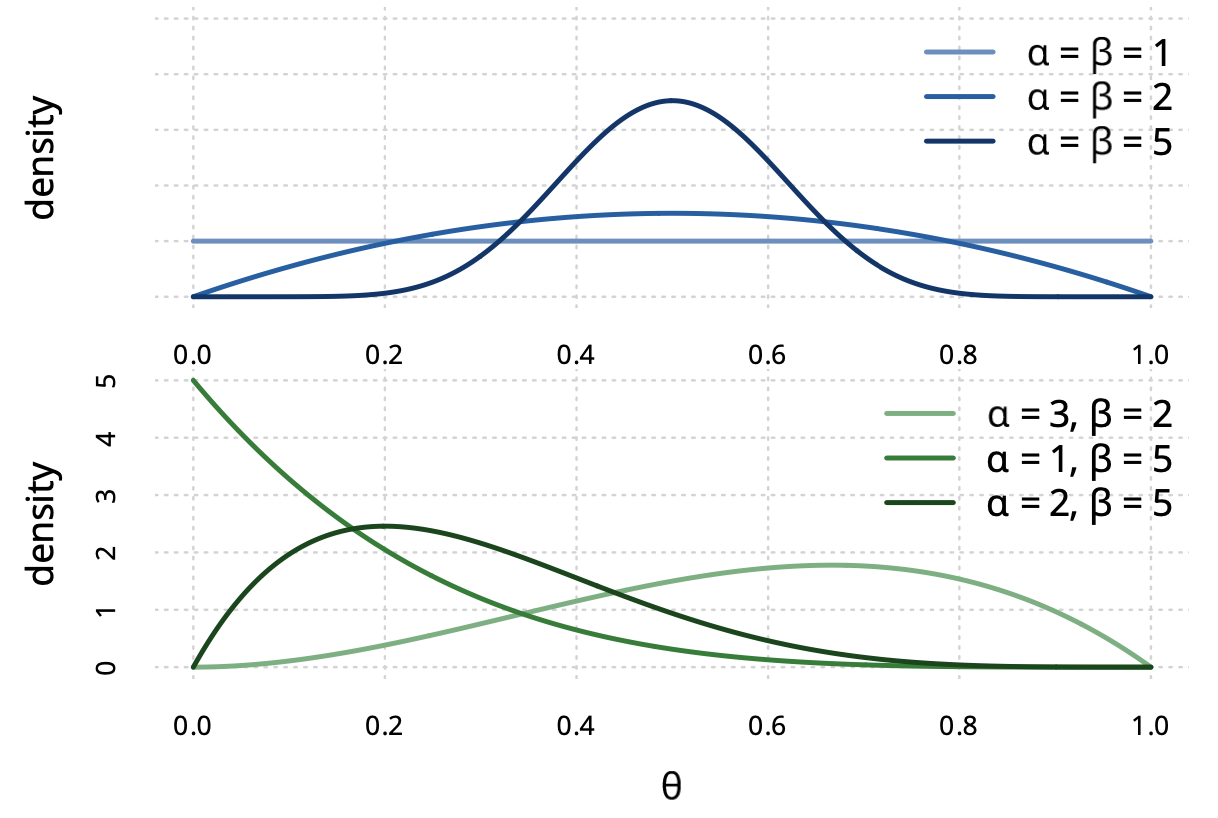
\includegraphics[width = 10cm]{betapdf.png}
\end{center}

The prior $p(\theta)$ determines which regions of the framework we believe to be relevant. Its choice is subjective, similarly to the likelihood. There are many approaches to choosing a sensible prior. Conjugate priors make the computation much easier. In this case, we used a conjugate Beta prior. A conjugate prior is a prior probability distribution that, when combined with a likelihood function through Bayes's theorem, produces a posterior distribution that is of the same family as the prior distribution. Setting $a_0 = b_0 = 1$ produces a uniform prior across the unit interval. 

Instead of $a_0$ and $b_0$, we can consider as parameters success probability $m_0 \approx \hat\theta_n = \frac{S_n}{n}$ and prior information $s_0 = a_0 + b_0$. These parameters are tied to the moments of the Beta distribution:

\[
	\E{\theta} = \frac{a_0}{a_0+b_0} = m_0, \qquad \Var{\theta} = \frac{\E{\theta}(1-\E{\theta})}{a_0 + b_0 + 1}.
\]

Our prior is then given by $\mathrm{Beta}(m_0s_0,(1-m_0)s_0)$.

\subsubsection{The Posterior}

Obtaining the posterior from combining the Bernoulli likelihood and the Beta prior, we get:

\begin{align*}
	p(\theta\mid\bm{y}) &\sim \mathrm{Beta}(a_n,b_n), \\
	a_n &= a_0 + S_n, \\
	b_n &= b_0 + n - S_n.
\end{align*}

The data enters only via two sufficient statistics, the number of successes, $S_n$, and the number of failures, $n-S_n$. 

We get this result by the following computation: A $\mathrm{Beta}(\alpha,\beta)$ density is, up to a constant, given by

\[
	f(\theta \mid \alpha,\beta) \propto \theta^{\alpha-1}(1-\theta)^{\beta-1}.
\]

We then get the posterior from Bayes's theorem, dropping factors independent of $\theta$ and matching moments to the Beta density:

\begin{align*}
	p(\theta\mid\bm{y}) &\propto p(\bm{y}\mid\theta)p(\theta) \\
	& \propto \theta^{S_n}(1-\theta)^{n-S_n} \quad \cdot \quad \theta^{a_0-1}(1-\theta)^{b_0 -1} \\
	& = \theta^{S_n+a_0-1}(1-\theta)^{n-S_n+b_0-1} \\
	\Rightarrow p(\theta\mid\bm{y}) &\sim \mathrm{Beta}(a_0+S_n,b_0+n-S_n).
\end{align*}

Using a uniform prior, this is how the posterior looks using different values of $n$ and $\frac{S_n}{n} = 0.05$:

\begin{center}
	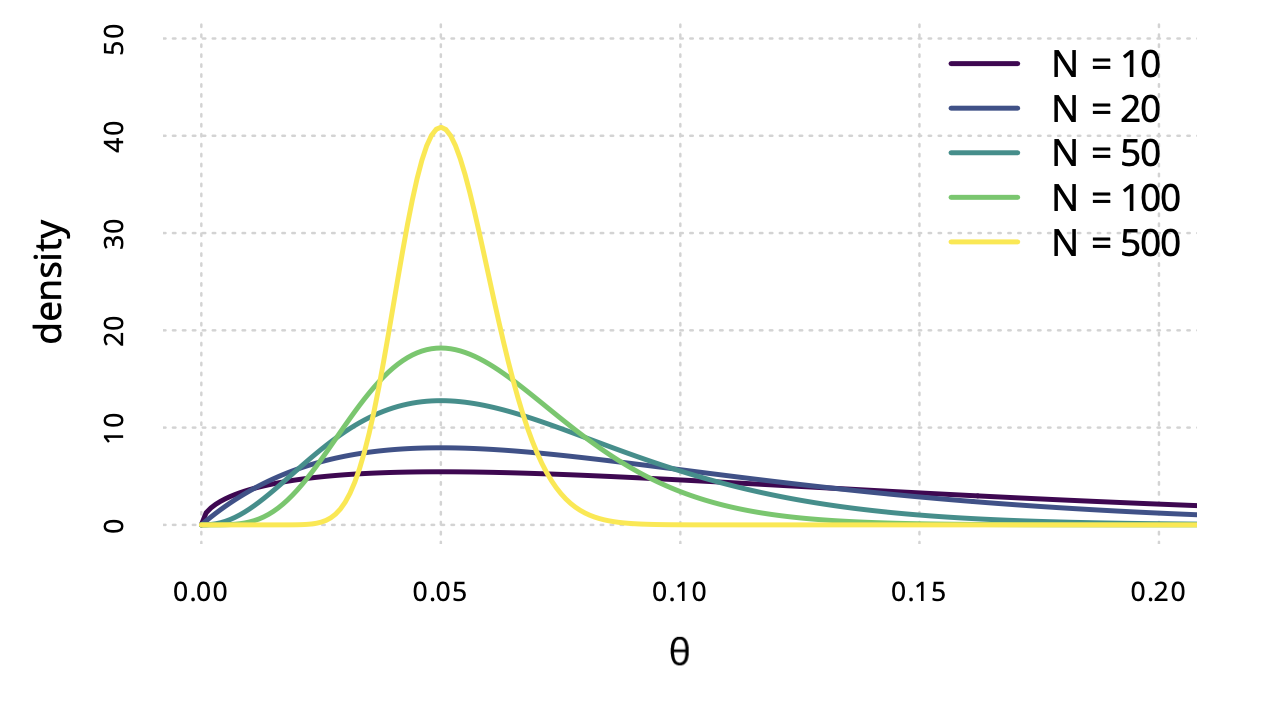
\includegraphics[width = 10cm]{betapost.png}
\end{center}

Using $m_0$ and $s_0$ as specified above as priors yields the following posteriors for $n = 50$ and $\frac{S_n}{n} = 0.05$:

\begin{center}
	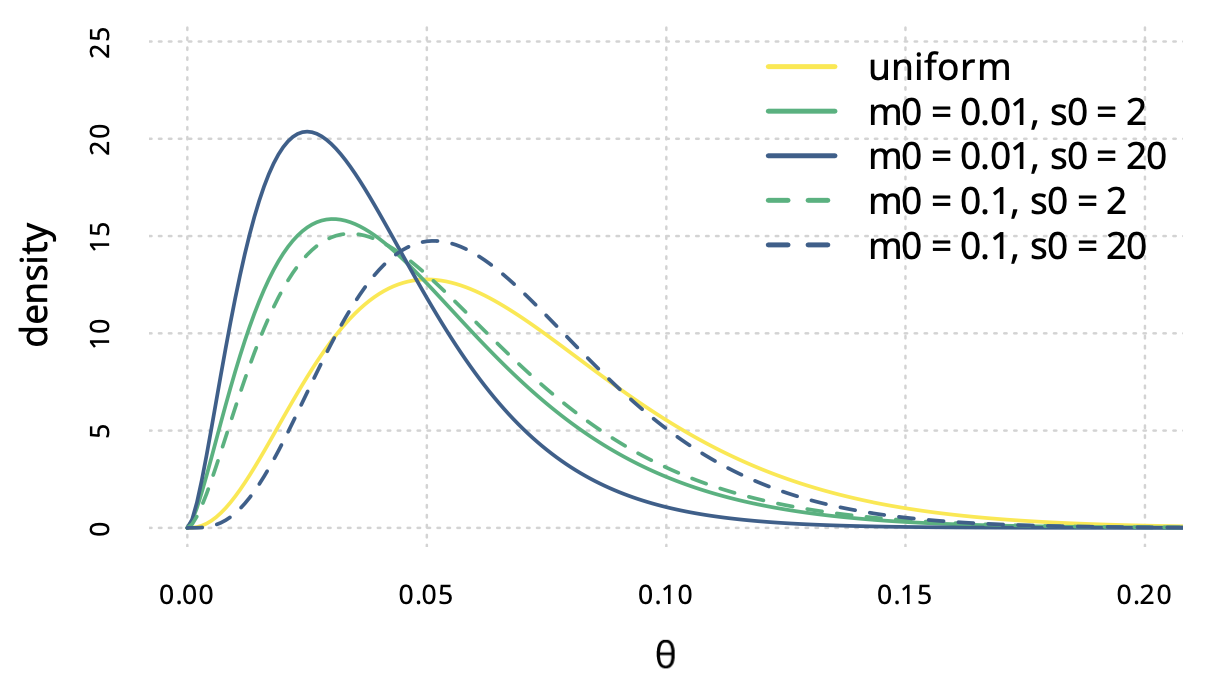
\includegraphics[width = 10cm]{betapost2.png}
\end{center}

From a full Bayesian analysis, we get a posterior density instead of just a point estimate. We can therefore obtain posterior moments and quantiles as well as any number of summary measures.

We can also get credible regions or credible intervals $C_\alpha$, which contain the parameter $\theta$ with probability $\alpha$. The highest posterior density region is the smallest region $C_\alpha$ for a given $\alpha$. 

\subsubsection{Summarizing the Posterior}

Summarizing the posterior using a simple number requires us to choose from multiple options, such as mode, median and mean.

\begin{center}
	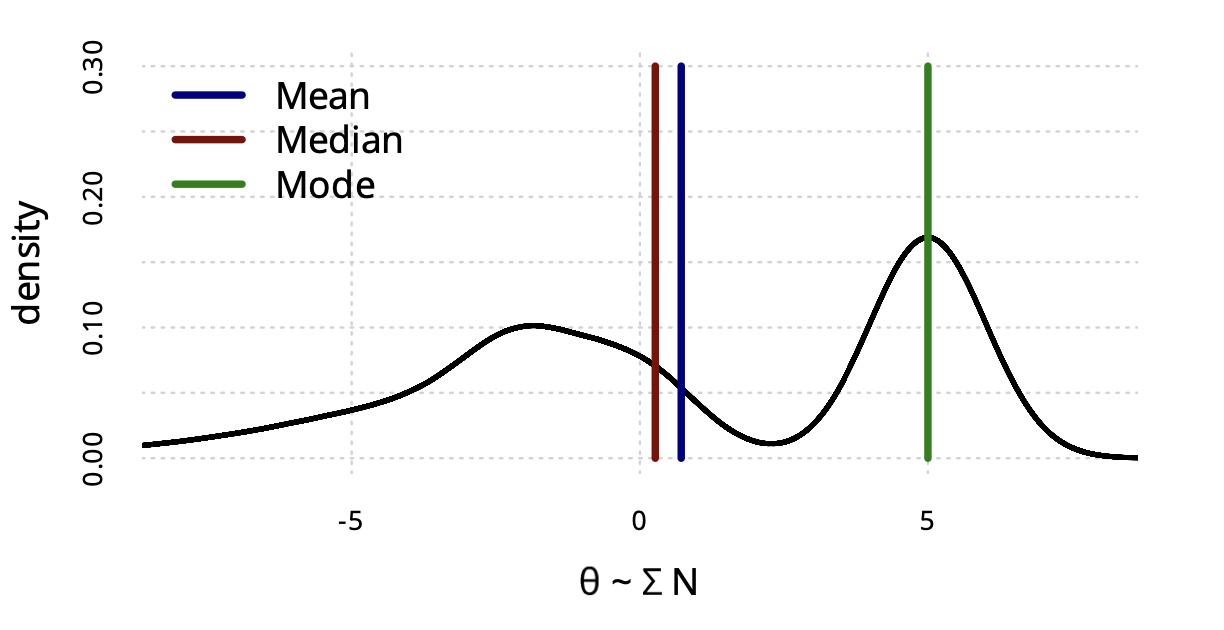
\includegraphics[width = 10cm]{posteriorpoint.png}
\end{center}

Even choosing an interval to cover 95\% probability is challenging. See this comparison between choosing the interval based on percentiles and choosing the HPD region:

\begin{center}
	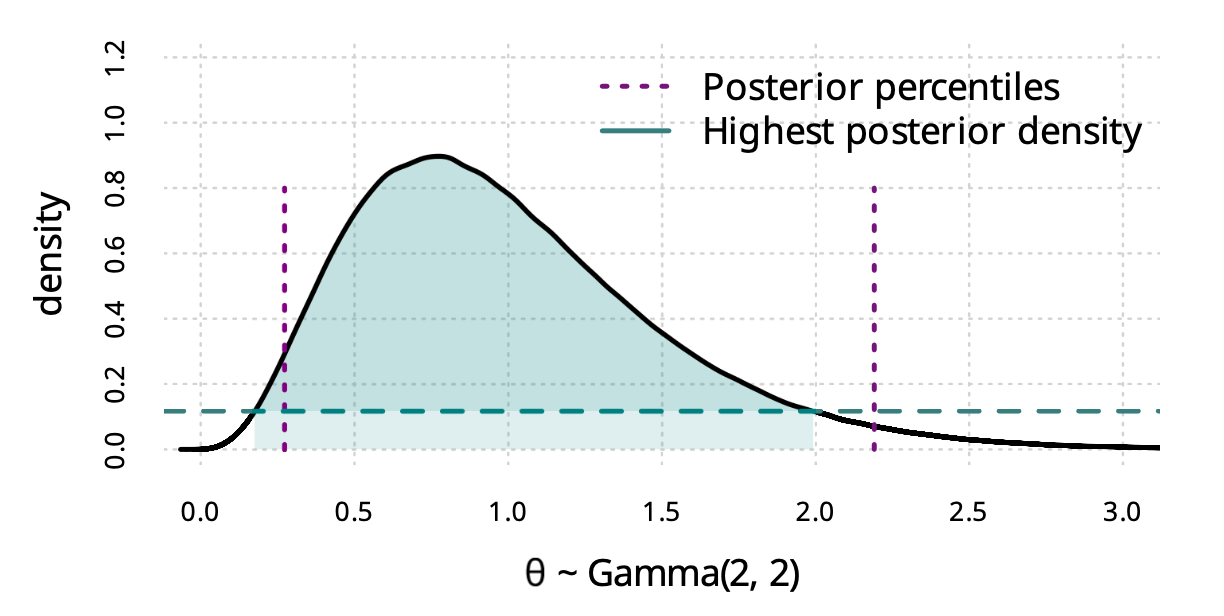
\includegraphics[width = 10cm]{posteriorregion1.png}
\end{center}

The HPD region can even be non-contiguous:

\begin{center}
	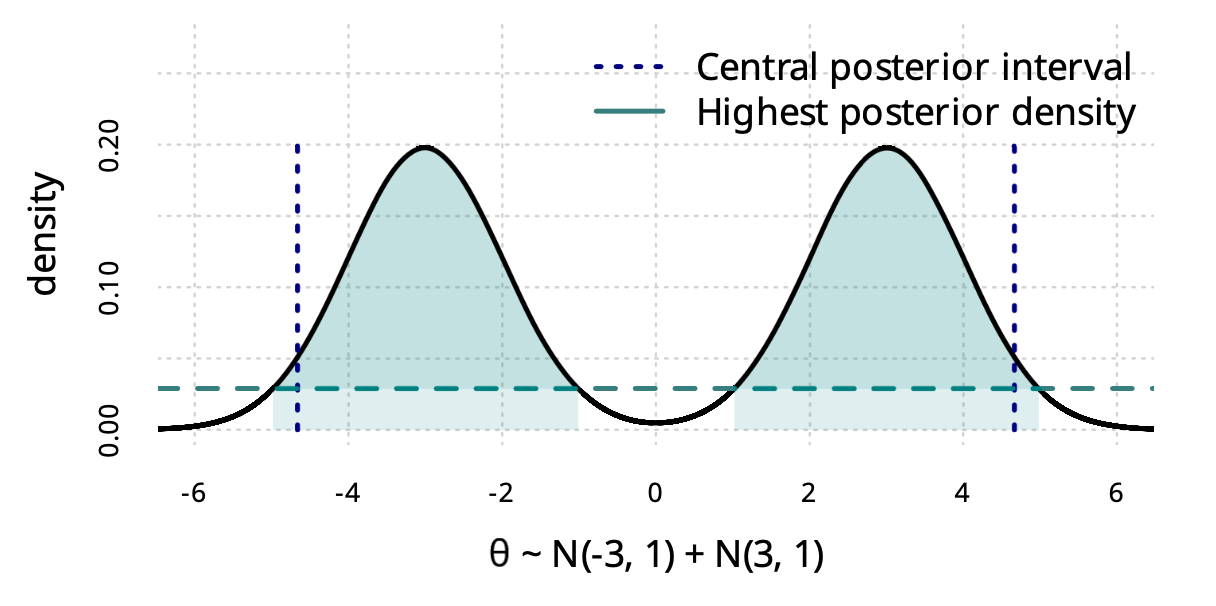
\includegraphics[width = 10cm]{posteriorregion2.png}
\end{center}

Posterior summaries are the core of Bayesian inference. In the case of the Beta posterior, moments are well-known and can be derived analytically. However, sometimes, we cannot derive them analytically or the posterior might not be of a well-known form. 

For a posterior summary, we essentially need the integral of a function $h(\cdot)$ of a parameter $\theta$:

\[
	\E{h(\theta)} = \int h(\theta)f(\theta)d\theta,
\]

where $\theta$ follows a distribution with density function $f(\theta)$. The posterior variance is given by:

\begin{align*}
	\Var{\theta\mid\mathcal{D}} &= \E{\theta\theta'\mid\mathcal{D}}-\E{\theta\mid\mathcal{D}}\E{\theta\mid\mathcal{D}}', \\
	\E{\theta\theta'\mid\mathcal{D}} &= \int (\theta\theta')p(\theta\mid\mathcal{D})d\theta, \\
	\E{\theta\mid\mathcal{D}} &= \int \theta p(\theta\mid\mathcal{D})d\theta.
\end{align*}

We can either compute this integral analytically if a closed-form solution exists, or we can use Monte Carlo integration if we can obtain samples $\theta^{(1)},\dots,\theta^{(S)}$ from $f$ like this:

\[
	\E{h(\theta)\mid\mathcal{D}} \approx \frac{1}{S}\sum^S_{s=1}h(\theta^{(s)}).
\]

If we can obtain samples, then the law of large numbers guarantees convergence of empirical moments to the moments of the probability distribution as $S\rightarrow \infty$.  If neither computing the integral analytically nor sampling from the distribution is possible, we can use Markov chain Monte Carlo methods.

% -----------------------------------------------------

\section{Bayesian Regression Analysis}

\subsection{Simple Linear Model}

\subsubsection{Setup}

The standard linear regression model is given by

\begin{equation}
	y_i = \bm{x}_i\bm{\beta} + \varepsilon_i, \qquad i = 1,\dots, n.
\end{equation}

Our distibutional assumption is with respect to the error term: $\varepsilon_i \sim \mathcal{N}(0,\sigma^2)\forall i$, and $\E{\bm{\varepsilon}\mid\bm{X}} = 0 \quad \Rightarrow \quad \E{\bm{y}\mid\bm{X}} = \bm{X\beta}$. The latent quantities in this model are $\bm{\beta}$, the regression coefficients, and $\sigma^2$, the error variance.

Assuming that there are no covariates, that is, $\bm{X} = \bm{1}$, we can express the model as 

\[
	y_i \sim \mathcal{N}(\beta,\sigma^2).
\]

Recall that a random variable $\theta \sim \mathcal{N}(\beta,\sigma^2)$ has the probability density function

\begin{equation}
	f(\theta\mid\mu,\sigma^2) = (2\pi\sigma^2)^{-1/2}\mathrm{exp}\left(-\frac{1}{2\sigma^2}(\theta-\mu)^2\right),
\end{equation}

where $\mu\in\mathbb{R}$ and $\sigma^2\in\mathbb{R}^{+}$ are parameters and the support is $\theta\in\mathbb{R}$. 

We want to learn about two free parameters, the mean $\beta$ and the variance $\sigma^2$. The likelihood function of our data is given by

\begin{align*}
	p(\bm{y}\mid\beta,\sigma^2) &= \prod^n_{i=1}p(y_i \mid \beta,\sigma^2) \\
	&= (2\pi\sigma^2)^{-n/2}\mathrm{exp}\left(-\frac{1}{2\sigma^2}\sum^n_{i=1}(y_i-\beta)^2\right).
\end{align*}

\subsubsection{Inference for $\sigma^2$ with $\beta$ known}

To get the conditional posterior $p(\sigma^2\mid\bm{y},\beta)$, we use Bayes's theorem. First, we consider the likelihood as a function of $\sigma^2$, meaning that we can drop constant values that do not depend on $\sigma^2$. We get

\[
	p(\bm{y}\mid\sigma^2,\beta) \propto (\sigma^2)^{-n/2+1-1}\mathrm{exp}\left(-\frac{1}{\sigma^2}\sum^n_{i=1}(y_i-\beta)^2/2\right).
\]

This is proportional to the PDF of an inverted Gamma distribution, $\theta\sim G^{-1}(c,d)$ with shape $c = n/2 + 1$ and rate $d = \sum^n_{i=1}(y_i-\beta)^2/2$. The density is given by

\[
	p(\theta\mid c,d) \propto (\theta)^{-c-1}\mathrm{exp}\left(-\frac{d}{\theta}\right).
\]

If we use an inverted Gamma prior for $\sigma^2$, that is, $\sigma^2\mid\beta \sim G^{-1}(c_0,d_0)$, then the prior and the likelihood are conjugate, and the posterior will also have the form of an inverted Gamma distribution. 

A random variable that is inverted-Gamma distributed, that is, $\theta\sim G^{-1}(\alpha,\beta)$, has the PDF

\begin{equation}
	f(\theta\mid\alpha,\beta) = \frac{\beta^\alpha}{\Gamma(\alpha)}\theta^{-\alpha-1}\mathrm{exp}\left(-\frac{\beta}{\theta}\right),
\end{equation}

where $\Gamma(\cdot)$ is the Gamma function and $\alpha\in\mathbb{R}^{+}, \beta\in\mathbb{R}^{+}$ are parameters. The support is $\theta\in\mathbb{R}^{+}$. 

The posterior of $\sigma^2$ with $\beta$ known is then 

\begin{align*}
	p(\sigma^2\mid\beta) &\propto p(\bm{y}\mid\sigma^2,\beta) \times p(\sigma^2\mid\beta) \\
	& \propto (\sigma^2)^{-n/2}\mathrm{exp}\left(-\frac{1}{2\sigma^2}\sum^n_{i=1}(y_i-\beta)^2\right)\times (\sigma^2)^{-c_0-1}\mathrm{exp}\left(-\frac{d_0}{\sigma^2}\right) \\
	& \propto (\sigma^2)^{-(n/2+c_0)-1}\mathrm{exp}\left(-\frac{1}{\sigma^2}\left(d_0 + \sum^n_{i=1}(y_i-\beta)^2/2\right)\right)
\end{align*}

This gives us the conditional posterior $p(\sigma^2\mid\bm{y},\beta)\sim G^{-1}(c_n,d_n)$, where 

\[
	c_n = c_0 + \frac{n}{2}, \qquad d_n = d_0 + \sum^n_{i=1}(y_i -\beta)^2/2.
\]

There are two sufficient statistics, $n$ and the variation around the mean, $\beta$. The following figure shows prior and posterior densities of $\sigma^2$ with increasing observations under an inverse Gamma prior, $G^{-1} (2,2)$, and data from a Normal with mean two and variance one:

\begin{center}
	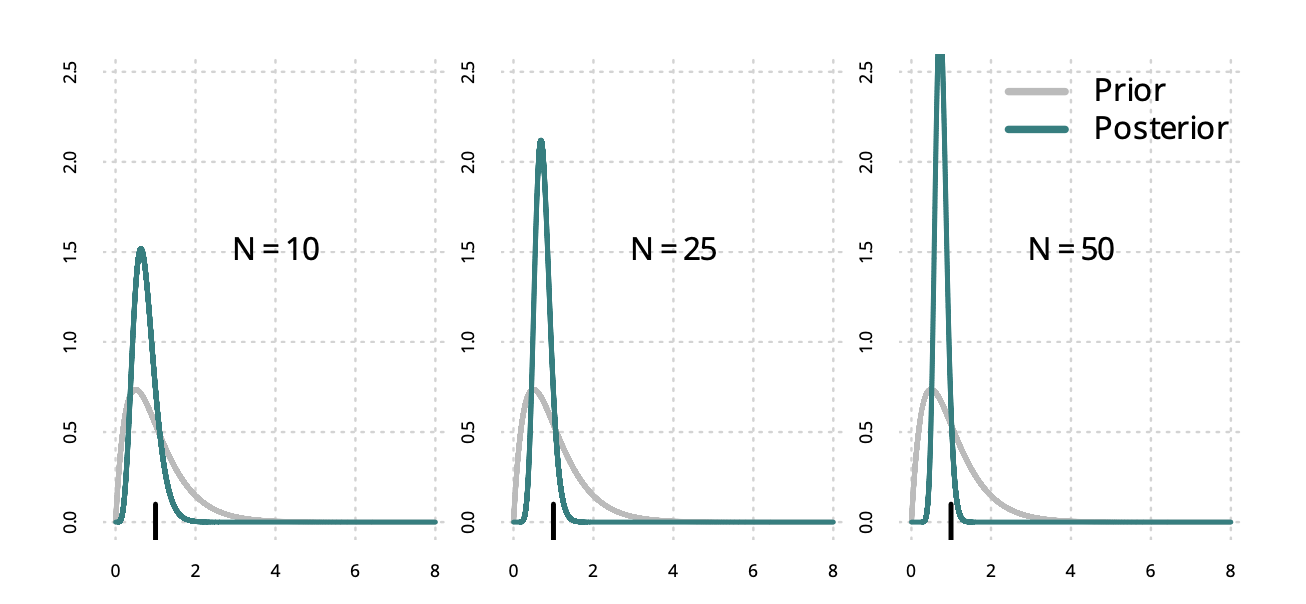
\includegraphics[width = 12cm]{inversegamma.png}
\end{center}

\subsubsection{Inference for $\beta$ with $\sigma^2$ known}

The likelihood $p(\bm{y}\mid\beta,\sigma^2)$, considered as a function of $\beta$, is proportional to:

\[
	p(\bm{y}\mid\beta,\sigma^2)  \propto \mathrm{exp}\left(-\frac{1}{2\sigma^2}\sum^n_{i=1}(y_i-\beta)^2\right).
\]

We can simplify this by using a variance decomposition to express the sum as

\[
	\sum^n_{i=1}(y_i-\beta)^2 = n(\beta-\bar{y})^2+(n-1)s^2,
\]

where $\bar{y}$ is the sample mean and $s^2$ is the bias-corrected sample variance. We can do this since

\begin{align*}
	\sum^n_{i=1}(y_i-\beta)^2 &= \sum^n_{i=1} (y_i-\bar{y}+\bar{y}-\beta)^2 \\
	&= \sum^n_{i=1}(y_i-\bar{y})^2+2(\bar{y}-\beta)\left(\sum^n_{i=1}(y_i-\bar{y})\right) + n(\bar{y}-\beta)^22 \\
	&=(n-1)s^2+0+n(\beta-\bar{y})^2.
\end{align*}

Using this variance decomposition, we can express the likelihood as

\[
	p(\bm{y}\mid\beta,\sigma^2) \propto \mathrm{exp}\left(-\frac{(\beta-\bar{y})^2}{2\sigma^2/n}\right). 
\]

This is proportional to the PDF of a normal distribution since

\[
	p(\theta\mid\mu,\varsigma) \propto \mathrm{exp}\left(\frac{(\theta-\mu)^2}{2\varsigma}\right).
\]

Under a flat prior $p(\beta) \propto \kappa$, the posterior is then given by $p(\beta\mid\bm{y},\sigma^2)\sim\mathcal{N}(\bar{y},\sigma^2/n)$. The sufficient statistics are $n$ and the sample mean, $\bar{y}$. The following figure shows prior and posterior densities of $\mu$ with increasing observations under a flat prior and data from a Normal with mean two and variance one.

\begin{center}
	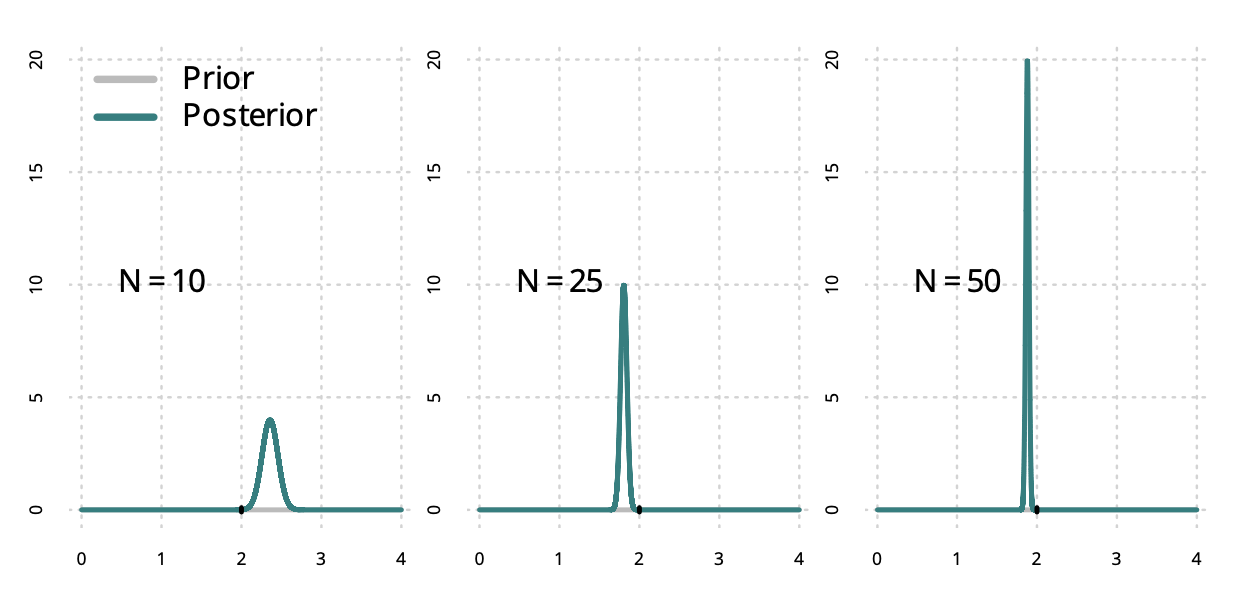
\includegraphics[width = 12cm]{normal.png}
\end{center}

\subsubsection{Inference on the Full Linear Regression Model}

In the previous, we derived the conditional posteriors $p(\sigma^2\mid\beta,\bm{y})$ and $p(\beta\mid\sigma^2,\bm{y})$ under the assumption that we know the other latent parameter. Now we need to derive the joint posterior distribution of $(\beta,\sigma^2)$ as well as the marginal posteriors $p(\sigma^2\mid\bm{y})$ and $p(\beta\mid\bm{y})$.

Using the variance decomposition, we can write the likelihood as 

\[
	p(\bm{y}\mid\beta,\sigma^2) = (2\pi\sigma^2)^{-n/2}\mathrm{exp}\left(-\frac{(n-1)s^2}{2\sigma^2}\right)\mathrm{exp}\left(\frac{(\beta-\bar{y})^2}{2\sigma^2/n}\right)
\]

If we use the improper prior $p(\beta,\sigma^2)\propto\sigma^{-2}$, an improper prior being a prior that does not integrate to one, we can derive the posterior:

\[
	p(\beta,\sigma^2\mid \bm{y}) \propto (\sigma^2)^{-\frac{n+1}{2}}\mathrm{exp}\left(-\frac{(n-1)s^2}{2\sigma^2}\right)\sigma^{-1}\mathrm{exp}\left(\frac{(\beta-\bar{y})^2}{2\sigma^2/n}\right)
\]

We can factor this posterior into two well-known densities by splitting it into the product of a conditional Normal density for $\beta\mid\sigma^2$, and a marginal inverted Gamma density for $\sigma^2$. There are three sufficient statistics, $n$, $\bar{y}$, and $s^2$. We have:

\[
	\beta\mid\bm{y},\sigma^2\sim\mathcal{N}(\mu_n,\Sigma_n\sigma^2),
\]

where $\mu_n = \bar{y}$ and $\Sigma_n = \frac{1}{n}$, and

\[
	\sigma^2\mid\bm{y}\sim G^{-1}(c_n,d_n),
\]

where $c_n = (n-1)/2$ and $d_n = (n-1)s^2/2$.

To find the marginal posterior of $\beta$, we need to solve the following integral:

\begin{align*}
	p(\beta\mid\bm{y}) &= \int_{\mathbb{R}^+}p(\beta,\sigma^2\mid\bm{y})d\sigma^2 \\
	&= \int_{\mathbb{R}^+}p(\beta\mid\sigma^2,\bm{y})p(\sigma^2\mid\bm{y})d\sigma^2.
\end{align*}

By integrating out $\sigma^2$, we find the following $t$ density:

\[
	p(\beta\mid\bm{y}) \sim t_{2c_n}(\mu_n,\Sigma_nd_n/c_n). 
\]

With the prior from before, $p(\beta,\sigma^2)\propto\sigma^{-2}$, this simplifies to $t_{n-1}(\bar{y},s^2/n)$. 

\subsubsection{Frequentist versus Bayesian Inference}

Frequentist confidence regions are based on 

\[
(\beta-\hat{\beta}) \sim t_v(0,\hat{\sigma}^2(\bm{X}'\bm{X})^{-1}),
\]

where $\hat{\beta} = (\bm{X}'\bm{X})^{-1}\bm{X}'\bm{y}$ and $\hat\sigma^2 = \bm{\varepsilon}'\bm{\varepsilon}/(n-k)$. Bayesians use the posterior:

\[
	p(\beta\mid\bm{y})\sim t_v(\hat\beta,\hat\sigma^2(\bm{X}'\bm{X}^{-1}) \quad\Rightarrow\quad (\beta-\hat\beta)\mid\bm{y}\sim t_v(0,\hat\sigma^2(\bm{X}'\bm{X})^{-1}).
\]

This implies that frequentist confidence regions can often (but not generally) be interpreted in a Bayesian sense.

\subsection{Standard Regression Analysis}

\subsubsection{Priors and Posteriors}

The standard linear regression model with multiple explanatory variables and spherical variance-covariance can be expressed as

\[
	\bm{y}\sim\mathcal{N}_n(\bm{X\beta},\sigma^2\bm{I}_n),
\]

where $\mathcal{N}_n$ denotes an $n$-dimensional multivariate Normal distribution, $n$ is the number of observations and $k$ is the number of explanatory variables. To draw inference on $\bm{\beta}\in\mathbb{R}^k$ and $\sigma^2\in\mathbb{R}^{+}$, we require the posterior distribution 

\[
	p(\bm{\beta},\sigma^2\mid\bm{y})\propto p(\bm{y}\mid\bm{\beta},\sigma^2)p(\bm{\beta},\sigma^2).
\]

The likelihood of the standard linear regression model is given by

\[
	p(\bm{y}\mid\bm{\beta},\sigma^2) = (2\pi\sigma^2)^{-n/2}\mathrm{exp}\left(-\frac{1}{2\sigma^2}(\bm{y}-\bm{X\beta})'(\bm{y}-\bm{X\beta})\right).
\]

As a function of $\sigma^2$, it equals the kernel of an inverted Gamma distribution. Thus, the (conditionally) conjugate prior for $\sigma^2$ is the IG distribution. As a function of $\bm{\beta}$, it is a quadratic form and mirrors the kernel of a multivariate Normal (MVN) distribution. The (conditionally) conjugate prior for $\bm{\beta}$ is thus the MVN distribution. A kernel, intuitively speaking, is the PDF with factors that ensure that the PDF integrates to one and are not functions of free variables omitted.

We can obtain a closed form posterior with the following prior:

\[
\beta \mid \sigma^2 \sim \mathcal{N}_k\left(\bm{\mu}_0, \sigma^2 \bm{\Sigma}_0\right), \quad \sigma^2 \sim \mathrm{G}^{-1}\left(c_0, d_0\right) .
\]

The joint posterior of $\left(\beta, \sigma^2\right)$ is then

\[
\beta\left|\sigma^2, \bm{y} \sim \mathcal{N}_k\left(\bm{\mu}_n, \sigma^2 \bm{\Sigma}_n\right), \quad \sigma^2\right| \bm{y} \sim \mathrm{G}^{-1}\left(c_n, d_n\right),
\]

where:

\begin{align*}
\bm{\mu}_n&=\bm{\Sigma}_n\left(\bm{\Sigma}_0^{-1} \bm{\mu}_0+\bm{X}^{\prime} \bm{y}\right),  &c_n&=c_0+n / 2 \\
\bm{\Sigma}_n&=\left(\bm{\Sigma}_0^{-1}+\bm{X}^{\prime} \bm{X}\right)^{-1},  &d_n&=d_0+\bm{S}_{\varepsilon} / 2 \text {, } \\
\bm{S}_{\varepsilon}&=\bm{y}^{\prime} \bm{y}+\bm{\mu}_0^{\prime} \bm{\Sigma}_0^{-1} \bm{\mu}_0-\bm{\mu}_n^{\prime} \bm{\Sigma}_n^{-1} \bm{\mu}_n \text {. } 
\end{align*}

\subsubsection{Sampling from the Joint Posterior Distribution}

If the joint posterior is available in closed form, we can obtain independent samples to visualize and draw inference. To do this and obtain $m=1,\dots,M$ samples $(\beta_{(m)},\sigma^2_{(m)})$, we first sample $\sigma^2_{(m)}$ from the marginal posterior and then use this to sample $\beta_{(m)}$ from the conditional posterior. 

We can express the posterior mean of our model as 

\begin{align*}
	\E{\beta\mid\bm{y}} &= (\Sigma_0^{-1}+\bm{X}'\bm{X})^{-1}(\Sigma_0^{-1}\mu_0+\bm{X}'\bm{X}\hat\beta) \\
	&= \bm{W}\Sigma_0^{-1}\E{\beta} + \bm{WX}'\bm{X}\hat\beta,
\end{align*}

where $\bm{W} = (\Sigma_0^{-1}+\bm{X}'\bm{X})^{-1}$ is the denominator of a weight matrix that depends on the prior information (or precision) $\Sigma_0^{-1}$ and the information matrix $\bm{X}'\bm{X}$. The posterior mean is therefore a weighted average of the prior mean $\E{\beta} = \mu_0$ and the OLS estimator $\hat\beta$.

Consider again the case where $\bm{X} = \bm{1}$ and therefore $\bm{X}'\bm{X} = n$. The posterior expectation of $\bm{\beta}$ is a weighted average of the sample mean $\bar y$ and the prior mean $\E{\beta} = \mu_0$:

\[
	\E{\beta\mid\bm{y}} = \frac{\Sigma_0^{-1}}{n+\Sigma_0^{-1}}\E{\beta}+\frac{n}{n+\Sigma_0^{-1}}\bar y.
\]

With increasing $n$, the effect of the prior disappears. The prior $p(\beta)$ imposes \textbf{shrinkage}, that is, the posterior expectation is pulled towards the prior expectation. Shrinkage priors can be understood as a Bayesian analogue to penalized estimators. The general idea is to shrink when there is not enough information in the data, and be agnostic otherwise.

\subsubsection{Multiple Regression with a Non-Conjugate Prior}

Before, we assumed that the prior covariance matrix of $\beta$ depends on $\sigma^2$. If we assume that $\beta$ and $\sigma^2$ are independent a priori, that is,

\[
	\beta\sim\mathcal{N}(\mu_0,\Sigma_0),\qquad\sigma^2\sim G^{-1}(c_0,d_0),
\]

where the prior covariance matrix $\Sigma_0$ directly controls shrinkage towards the prior mean, then we get a joint posterior that does not have a well-known closed form. There is, however, a closed form for the conditional posteriors:

\[
	\beta\mid\sigma^2,\bm{y}\sim\mathcal{N}_k(\mu_n,\Sigma_n),\qquad \sigma^2\mid\beta\bm{y}\sim G^{-1}(c_n,d_n),
\]

where 

\begin{align*}
	\mu_n &= \Sigma_n(\Sigma_0^{-1}\mu_0+ \bm{X}'\bm{y}/\sigma^2), \\
	\Sigma_n &= (\Sigma_0^{-1}+\bm{X}'\bm{X}/\sigma^2)^{-1}, \\
	c_n &= c_0 + n/2, \\
	d_n &= d_0 + \bm{\varepsilon}'\bm{\varepsilon}/2, \\
	\bm{\varepsilon} &= \bm{y}-\bm{X\beta}.
\end{align*}

Previously, we have used conjugate priors, such that the posterior is from the same distribution family as the prior. This meant that we could directly compute many quantities of interest, and obtain independent samples from the posterior, which we used to compute arbitrary quantities of interest. Now, the posterior has no simple analytical form and
we cannot produce independent samples from $p(\beta,\sigma^2\mid\bm{y})$. However, we can produce dependent samples.


% -----------------------------------------------------

\section{Bayesian Estimation}

\subsection{Numerical Integration}

We want to learn about the posterior $p(\theta\mid\mathcal{D})$ from 

\[
	p(\theta\mid\mathcal{D})\propto p(\mathcal{D}\mid\theta)p(\theta).
\]

In some cases, we know the posterior distribution and some summaries of interest, generally however, we do not. We therefore need numerical integration methods to summarize the posterior. If we can obtain samples from our posterior density, $f(\theta)$, we can use probabilistic \textbf{Monte Carlo integration}, where we do the following:

\begin{enumerate}
	\item Draw samples $(\theta^{(1)},\dots,\theta^{(S)})$,
	\item Compute the desired function, $h(\theta^{(s)})$, for each sample,
	\item Use the results to compute a summary, such as the expected value.
\end{enumerate}

The sampling error decreases as $S$ increases.

\subsection{Markov Chain Monte Carlo}

MCMC Methods allow sampling from any distribution. The idea is that we construct a Markov chain that has the desired distribution as its stationary distribution. We can then obtain samples from the desired distribution by taking states from the Markov chain.

A Markov chain process is a memoryless stochastic process. We can define it as a sequence of random variables that satisfies this property:

\[
	p(x_{t+1}\mid x_t, x_{t-1}, \dots, x_0) = p(x_{t+1}\mid x_t)\forall t,
\]

where $x_t$ is the state of the chain at time $t$ and $p(x_{t+1}\mid x_t)$ is the transition probability. A Markov chain can be fully characterized by an initial state $x_0$, a state space $\mathcal{X}$, and transition probabilities. The function $K(a,b)$ that gives the probability of transition to $b$ given a state $a$ is called the transition kernel:

\[
	K(a,b) = p(x_{t+1}=b \mid x_t = a),\qquad a,b\in \mathcal{X}.
\]

Markov Chains with discrete state space have a transition kernel that can be represented as a matrix. The Markov chain is stationary if $\rho((K))<1$, where $\rho(\cdot)$ denotes the spectral radius, that is, the maximal absolute value of the eigenvalues. However, in a simple autoregressive model like this:

\[
	y_t = \rho y_{t-1} + \varepsilon_t, \qquad \varepsilon_t\sim\mathcal{N}(0,1),
\]

the state space is $\mathcal{X} \in \mathbb{R}$ and the transition kernel is

\[
	K(a,b) = \frac{1}{\sqrt{2\pi}}\mathrm{exp}\left(-\frac{(b-\rho a)^2}{2}\right).
\]

\subsection{Gibbs Sampler}

Before, we imposed independent Normal and Inverse Gamma priors. We need to know the joint posterior $p(\beta, \sigma^2\mid\bm{y})$, but only know the conditional posteriors $p(\beta\mid\sigma^2,\bm{y})$ and $p(\sigma^2\mid\beta, \bm{y})$. The Gibbs sampler, an MCMC algorithm, sequentially generates values from each of the conditional distributions, conditional on current other values. This sequence is a Markov chain with the desired joint distribution as its stationary distribution. It can be visualized like this:

\begin{center}
	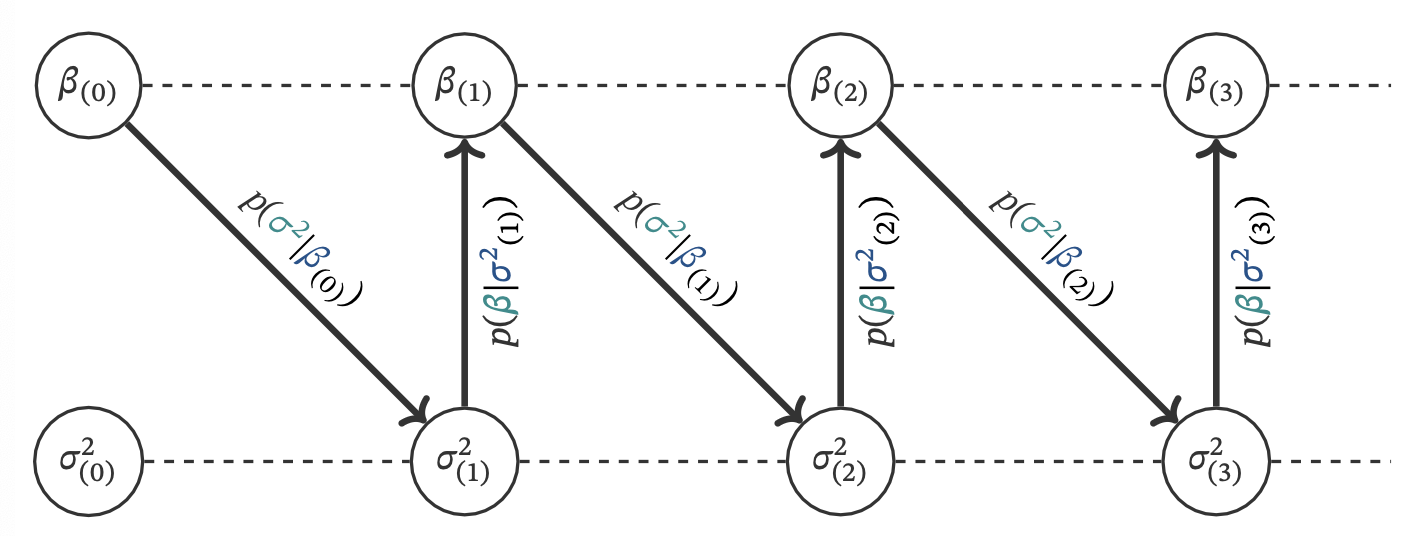
\includegraphics[width = 12cm]{gibbs.png}
\end{center}

In general, for a latent that can be divided into two blocks $\theta = (\theta^1,\theta^2)$, we can use a \textbf{two-block Gibbs sampling algorithm}. We start with a starting value $\theta^2_{(0)}$. Then, we iterate for $s = 1, \dots, S$:

\begin{enumerate}
	\item We sample $\theta^1_{(s)}$ from the conditional distribution $p(\theta^1\mid\theta^2_{(s-1)},\mathcal{D})$,
	\item We sample $\theta^2_{(s)}$ from the conditional distribution $p(\theta^2\mid\theta^1_{(s)},\mathcal{D})$.
\end{enumerate}

We then discard the first $S_0$ draws as burn-in, such that the sampler has converged to the joint distribution. The transition kernel is $K(\theta_{\text{new}},\theta_{\text{old}}) = p(\theta^1_\text{new}\mid\theta^2_\text{new},\mathcal{D})p(\theta^2_\text{new}\mid\theta^1_\text{old})$. 

That Gibbs sampler is a special case of the Metropolis-Hastings algorithm where draws are always accepted. The idea of the MH algorithm is to 

\begin{enumerate}
	\item Propose a new draw from $q(\theta_\text{new}\mid\theta_\text{old})$,
	\item Accept the new value with probability $\alpha(\theta_\text{new}\mid\theta_\text{old})$:
	
	\[
		\alpha(\theta_\text{new}\mid\theta_\text{old}) = \mathrm{min}\left(1,\frac{p(\theta_\text{new}\mid\mathcal{D})q(\theta_\text{old}\mid\theta_\text{new})}{p(\theta_\text{old}\mid\mathcal{D})q(\theta_\text{new}\mid\theta_\text{old})}\right)
	\]
\end{enumerate}

MH samplers do not rely on well-known conditional distributions. They only need a function that is proportional to the target distribution.

\subsection{Convergence}

The stationary distribution of the Gibbs sampler \textbf{converges} to the joint distribution under relatively mild assumptions. The choice of the starting value is deterministic, but can only distort inference if we obtain only few samples. The aforementioned burn-in period helps in limiting the impact of the starting value. To assess convergence, we can use convergence checks and multiple chains with different starting values. Plots we can use for convergence checks include trace plots, density plots and QQ plots.

MCMC Algorithms are approximate. We want to know whether the samples are representative of the distribution and how effective the sampler is at exploring the distribution. These issues refer to the \textbf{mixing} of the Markov chain. A sampler mixes well if it explores the full distribution (i.e., not only certain areas) effectively (i.e., with low autocorrelation).

MCMC draws are autocorrelated since they are dependent on earlier draws. Dependent samples are less informative than independent ones. To assess this inefficiency, we can use the effective sample size:

\[
	\mathrm{ESS} = \frac{m}{\tau},
\]

where $m$ is the sample size, and $\tau$ is a scaling factor, such as $1+2\sum\rho(l)$, where $\rho(l)$ is the autocorrelation at lag $l$.

To address poor mixing, we can increase the number of draws, change the sampler, improve the sampler, use block sampling, reparameterize models or work out a closed form.


% -----------------------------------------------------

\section{Model Selection and Priors}

\subsection{Bayesian Hypothesis Testing}

For Bayesian "testing," we can use the probability that the latent $\theta$ lies in a subset of the parameter space $C$ given the data $\mathcal{D}$:

\begin{equation}
	\int_C p(\theta\mid\mathcal{D})d\theta.
\end{equation}

Thus, we can directly determine the posterior probability of a hypothesis by computing the integral:

\begin{center}
	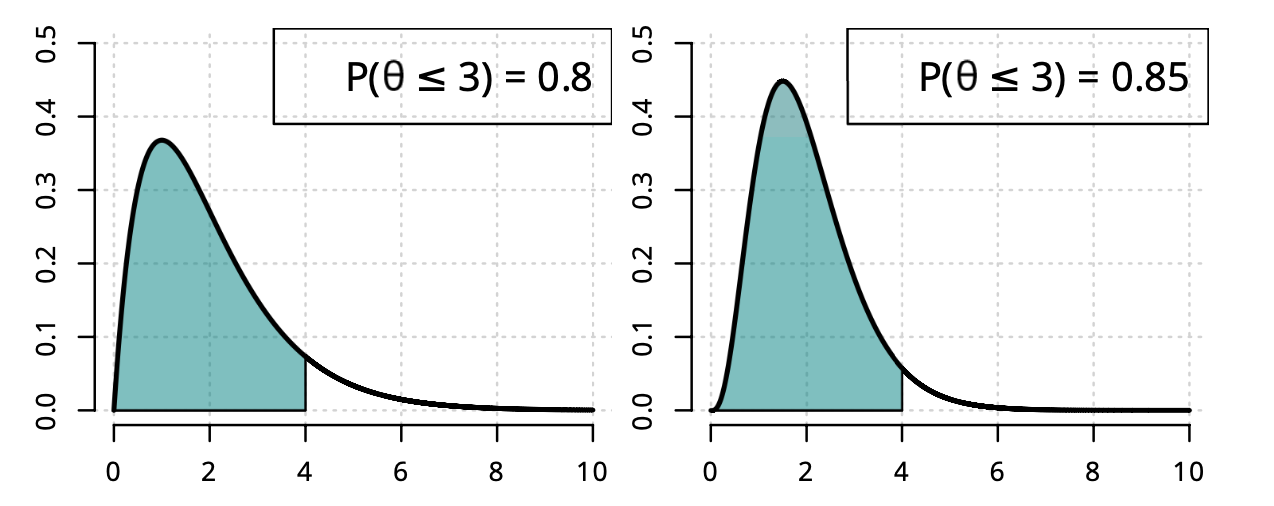
\includegraphics[width=12cm]{posteriorhypothesis.png}
\end{center}

We have strong evidence for a hypothesis $H_a:\theta \leq \theta_0\mid \mathcal{D}$ if $P(\theta\leq \theta_0\mid\mathcal{D}) \gg P(\theta > \theta_0\mid\mathcal{D})$. We select a null hypothesis, thereby expressing prior belief in the null, and reject it if the data is in conflict with it. With Bayesian testing, we get a probability directly. With frequentist testing, we get a "yes" or "no" answer that is correct with a certain probability.

\subsection{Model Selection}

Assume we have $m$ models $M_1,\dots,M_k$ to explain our data $\mathcal{D}$. These models are characterized by their latent parameters $\theta_j$, the conditional likelihood $p(\mathcal{D}\mid\theta_j,M_j)$, and the conditional prior $p(\theta_j\mid M_j)$. We can go about different ways in the selection of a model to settle on.

\subsubsection{Bayesian Model Selection}

We consider each model to arise from a discrete model space and assign prior probabilities $P(M_j)$ to each model. We then compute the posterior probabilities $P(M_j\mid\mathcal{D})$ over the model space:

\begin{equation}
	P(M_j\mid\mathcal{D}) \propto P(\mathcal{D}\mid M_j)P(M_j) \qquad \forall j \in 1,\dots, k,
\end{equation}

where $P(\mathcal{D}\mid M_j)$ is the marginal likelihood of model $M_j$, $P(\mathcal{D}\mid M_j) = \int_{\Theta_m}p(\mathcal{D},\theta_j\mid M_j)d\theta_j = \int_{\Theta_m}p(\mathcal{D}\mid\theta_j,M_j)p(\theta_m\mid M_j)d\theta_j$.

Let $R(M_j,M)$ be a loss function for selecting the model $M_j$ when $M$ is the true model. We can determine the expected loss of selecting a model for each candidate:

\begin{equation}
	\E{R(M_j)\mid \mathcal{D}} = \sum^k_{j = 1}R(M_j,M)P(M\mid \mathcal{D}).
\end{equation}

We can then select the model with the lowest expected loss. The 0/1 loss function is given by

\[
	r(M_j,M) = 
	\begin{cases}
		0, &\text{ if }M_j = M, \\
		1, & \text{ otherwise.}
	\end{cases}
\]

Let $M_{j^*}$ be the true model. Then the expected risk is 

\[
	\E{R(M_j) \mid \mathcal{D}} = \sum^k_{j = 1,j \neq j^*}P(M_{j^*}\mid \mathcal{D}) = 1 - P(M_j\mid \mathcal{D}).
\]

We minimize risk (the expected loss) by choosing the model with the highest posterior probability. If all models have the same prior probability, this loss function selects the model with highest marginal likelihood.

The \textbf{candidate's formula} is given by 

\begin{equation}
	p(\mathcal{D}\mid M)  = \frac{p(\mathcal{D}\mid\theta)p(\theta \mid M)}{p(\theta\mid \mathcal{D}, M)}.
\end{equation}

If the posterior density comes from a well-known distribution family, we can compute the marginal likelihood explicitly -- it is equal to the normalizing constant of the posterior density:

\[
	p(\theta\mid\mathcal{D}) = \frac{p(\mathcal{D}\mid\theta)p(\theta)}{p(\mathcal{D})}.
\]


For a computational example, consider data from the Poisson distribution, $y_i \overset{\mathrm{iid}}{\sim} P(\mu)$, and the conditionally conjugate Gamma prior, $\mu \sim G\left(a_0, b_0\right)$. We can solve the integration for the marginal likelihood of a model $M_1$ analytically:

\begin{align*}
p\left(\bm{y} \mid M_1\right) & =\int_0^{\infty} p\left(\bm{y} \mid \mu, M_1\right) p\left(\mu \mid M_1\right) d \mu, \\
& =\frac{\left(\bm{y} \mid \mu, M_1\right) p\left(\mu \mid M_1\right)}{p\left(\mu \mid \bm{y}, M_1\right)}=\frac{b_0^{a_0} \Gamma\left(a_n\right)}{b_n^{a_n} \Gamma\left(a_0\right) \prod_{i=1}^n \Gamma\left(y_i+1\right)}
\end{align*}

where $a_n=a_0+\sum y_i$ and $b_n=b_0+n$ are the sufficient statistics for the posterior of $\mu \mid \bm{y}, M_1 \sim \mathrm{G}\left(a_n, b_n\right)$.

Now consider an alternative model with a structural break, where we have $y_i\overset{\mathrm{i i d}}{ \sim} {P}\left(\mu_j\right)$, with

\[
\mu_j=\left\{\begin{array}{l}
\mu_1 \text { if } i<i_0 \\
\mu_2 \text { if } i \geq i_0
\end{array}\right.
\]

With conditionally conjugate priors, $\mu_1 \sim G\left(a_0, b_0\right), \mu_2 \sim G\left(a_0, b_0\right)$, such that $\mathrm{E}\left(\mu_1-\mu_2\right)=0$, the marginal likelihood is:

\begin{align*}
p\left(\bm{y} \mid M_2\right) & =\frac{\left(\bm{y} \mid \mu_1, \mu_2, M_2\right) p\left(\mu_1, \mu_2 \mid M_2\right)}{p\left(\mu_1, \mu_2 \mid \bm{y}, M_2\right)} \\
& =\frac{b_0^{2 a_0} \Gamma\left(a_{n, 1}\right) \Gamma\left(a_{n, 2}\right)}{b_{n, 1}^{a_{n, 1}} b_{n, 2}^{a_{n, 2}} \Gamma\left(a_0\right) \prod_{i=1}^n \Gamma\left(y_i+1\right)},
\end{align*}

where $a_{n, 1}=a_0+n_1 \overline{\bm{y}}_1, b_{n, 1}=b_0+n_1$ (and analogously $a_{n, 2}, b_{n, 2}$ ) are sufficient statistics for the posterior of $\mu_1, \mu_2 \mid \bm{y}, M_2$.

The \textbf{Bayes factor} is the odds ratio of two marginal likelihoods:

\begin{align*}
\mathrm{BF} & =\frac{p\left(\mathcal{D} \mid M_1\right)}{p\left(\mathcal{D} \mid M_2\right)}, \\
& =\frac{\int p\left(\mathcal{D} \mid \theta_1, M_1\right) p\left(\theta_1 \mid M_1\right) d \theta_1}{\int p\left(\mathcal{D} \mid \theta_2, M_2\right) p\left(\theta_2 \mid M_1\right) d \theta_2}=\frac{p\left(M_1 \mid \mathcal{D}\right) p\left(M_2\right)}{p\left(M_2 \mid \mathcal{D}\right) p\left(M_1\right)}
\end{align*}

For the example from before, we have:

\[
\mathrm{BF}=\frac{\Gamma\left(a_0\right)}{b_0^{a_0}} \times \frac{\Gamma\left(a_n\right)}{\Gamma\left(a_{n, 1}\right) \Gamma\left(a_{n, 2}\right)} \times \frac{b_{n, 1}^{a_{n, 1}} b_{n, 2}^{a_{n, 2}}}{b_n^{1_n}} .
\]

Exact computation of the marginal likelihood is not possible for many interesting models, and numerical integration can be very challenging computationally. Models to approximate it are bridge sampling and importance sampling. Model space MCMC methods, such as stochastic search variable selection (SSVS) are an alternative approach. When comparing models using the marginal likelihood, it is important to consider the potentially strong influence of priors and their parameters.

The standard linear regression model, $\bm{y} \sim \mathcal{N}(\bm{X\beta},\sigma^2\bm{I})$ with conjugate priors and closed form posteriors 

\begin{align*}
	\beta\mid\sigma^2\sim\mathcal{N}(\mu_0,\sigma^2\Sigma_0), &\qquad\sigma^2\sim G^{-1}(c_0,d_0), \\
	\beta\mid\sigma^2,\bm{y} \sim \mathcal{N}(\mu_n,\sigma^2\Sigma_n), &\qquad \sigma^2\mid\bm{y}\sim G^{-1}(c_n,d_n),
\end{align*}

has, by the candidate's formula, the following marginal likelihood:

\begin{align*}
	p(\bm{y}\mid M) &= \frac{\Gamma(c_n)(d_0)^{c_0}|\Sigma_n|^{0.5}}{\Gamma(c_0)(d_n)^{c_n}|\Sigma_0|^{0.5}(2\pi)^{n/2}} \\
	&= |\Sigma_0^{-1}|^{0.5}\times \frac{d_0^{c_0}}{\Gamma(c_0)}\times \frac{\Gamma(c_n)|\Sigma_n|^{0.5}}{(d_n)^{c_n}} \times \frac{1}{(2\pi)^{n/2}}.
\end{align*}

By \textbf{Lindley's paradox}, as the prior is becoming more and more vague, the simpler model will be chosen with probability 1, regardless of the data $\mathcal{D}$, the sample size $n$, and the true model. Prior distributions for parameters that appear only in some models should therefore not be vague.

\subsubsection{Variable Selection for Regression Models}

Consider the standard regression model 

\[
	\bm{y}\sim\mathcal{N}_n(\bm{X\beta},\sigma^2\bm{I}_n)
\]

with $k$ covariates. To answer which of the $k$ covariates we should include, we can either compute all $P(M_j\mid\mathcal{D})$ and choose the model with the highest posterior probability, or use an approximation (which penalizes models with many parameters), sich as the Bayesian Information Criterion:

\begin{equation}
	\mathrm{BIC} = -2\ell + k\:\mathrm{ln}\:n.
\end{equation}

For standard regression models, the marginal likelihood and the Bayesian Information Criterion are closely related if the number of observations is large.

It would be highly computationally intensive to compute the ML or BIC for all possible models since there are $m = 2^{k-1}$ possible models to compare. The idea of \textbf{Model space MCMC} is therefore to sample models according to their posterior probability. We search for models stochastically, and model probabilities are estimated by their relative frequency. More promising models are visited more often, while models with low probability are usually not visited. One method for this is \textbf{stochastic search variable selection} (SSVS). The idea of SSVS is to extend the standard linear model with indicators $\delta_j$ for each element of $\bm{\beta}$ such that

\[
	\beta_j = 
	\begin{cases}
		0 & \text{ if } \delta_j = 0 \\
		\text{unrestricted} & \text{ if } \delta_j = 1.
	\end{cases}
\]

The full model is then given by

\[
	y_i = \delta_1 x_{i1}\beta_1 + \dots + \delta_k x_{ik}\beta_k + \varepsilon_i.
\]

MCMC estimation of the SSVS model is then conceptually straightforward. These samplers are sometimes called model choice MCMC (MC3). We proceed as follows:

\begin{enumerate}
	\item \textbf{Model Search}: Sample a new indicator $\delta$. Sample $\delta_j$ from $p(\delta_j\mid\delta_{-j},\bm{y})$ for all $j$. 
	\item \textbf{Parameter Estimation}: Sample non-zero elements of $\beta$ and $\sigma^2$ conditional on $\delta$ from $p(\beta,\sigma^2\mid\delta,\bm{y})$ using standard methods. 
\end{enumerate}

With a Gibbs sampler, we sample elements $\delta_j$ in blocks from their discrete, conditional posteriors,

\begin{align*}
	P(\delta_j = 0 \mid \delta_{-j},\bm{y}) &\propto p(\bm{y}\mid\delta_j = 0, \delta_{-j})p(\delta_j = 0\mid \delta_{-j}), \\
	P(\delta_j = 1 \mid \delta_{-j},\bm{y}) &\propto p(\bm{y}\mid\delta_j = 1, \delta_{-j})p(\delta_j = 1\mid \delta_{-j}).
\end{align*}

The probabilities $P(\delta_j = 0 \mid \delta_{-j},\bm{y})$ and $P(\delta_j = 1 \mid \delta_{-j},\bm{y})$ need to be normalized before sampling. 

A simple prior for the indicator $\delta$ is to assume a fixed proportion $\pi$ of non-zero coefficients:

\[
	P(\delta_j = 1 \mid \pi) = \pi.
\]

This implies a binomial distribution on the model size $k_\delta$:

\[
	k_\delta = \sum^k_{i=1}\delta_i\sim\mathrm{Binom}(k,\pi).
\]

With $\pi = 0.5$, we have a uniform prior over all models, i.e., we are uninformative with respect to the model. However, this prior is highly informative on the model size $k_\delta$. To induce a uniform prior over the model \textit{size}, we can use a hierarchical prior, where $\pi \sim U[0,1]$. For large models, this is preferable to fixing $\pi$. 

Assume, for example, that there is one good model with $\delta^*$ out of $2^{20}$, such that $p(\bm{y}\mid\delta^*) = \mathrm{BF} p(\bm{y}\mid \delta_m)$, where $\mathrm{BF}>1$:

\begin{align*}
	p(\delta^*\mid\bm{y}) &= \frac{p(\bm{y}\mid \delta^*)p(\delta^*)}{p(\bm{y}\mid \delta^*)p(\delta^*) + \sum_{\delta_j\neq\delta^*}p(\bm{y}\mid\delta_j)p(\delta_j)} \\
	&= \frac{\mathrm{BF}}{\mathrm{BF} + (2^{20}-1)} \approx \frac{\mathrm{BF}}{\mathrm{BF} + 1{,}000{,}000}.
\end{align*}

\subsection{Other Approaches}

An alternative to looking for the "best model" and thereby ignoring uncertainty around the model selection is to consider all candidate models, weighted by their posterior probability. This approach is called \textbf{Bayesian model averaging} (BMA). Instead of conditioning parameters on one model, we now keep all parameter estimates and weigh them. 

Priors that zero-out unwanted parameters are called spike-and-slab priors. We can express them using a mixture of normals,

\[
	p(\beta\mid\delta)\sim \delta\mathcal{N}(0,v_1) + (1-\delta)\mathcal{N}(0,v_2),
\]

where $v_1\gg v_2$, meaning that we pull $\beta$ towards zero if $\delta= 0$. The mixture of normals can be visualized like this:

\begin{center}
	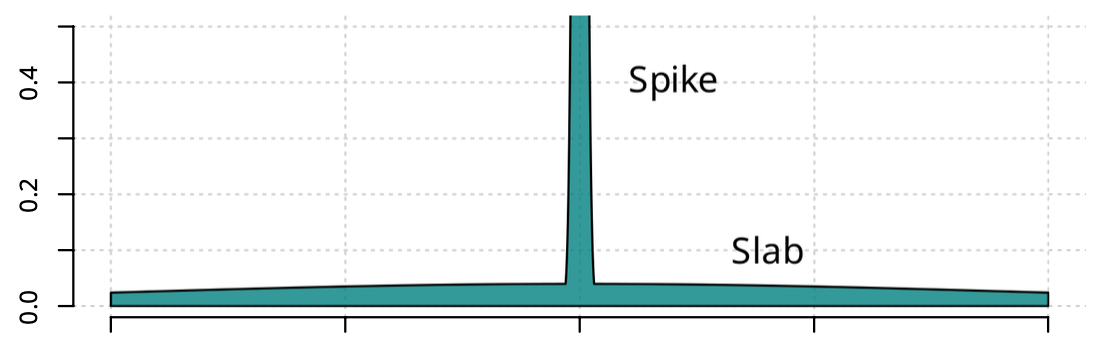
\includegraphics[width = 12cm]{spikeslab.png}
\end{center}

Another approach are continuous shrinkage priors, which are similar to frequentist regularized estimators. Examples are Bayesian LASSO, where

\[
	p(\beta\mid\tau_j^2)\sim\mathcal{N}\left(0,\frac{2}{\lambda^2}\tau^2_j\right), \qquad \tau_j^2\sim\mathcal{E}(1),
\]

or the Normal-Gamma prior, where

\[
	p(\beta\mid\tau_j^2) \sim\mathcal{N}\left(0,\frac{2}{\lambda^2}\tau_j^2\right), \qquad \tau^2_j \sim G(a_\tau,a_\tau).
\]

In priors like these, the term $2/\lambda^2$ applies global shrinkage, while $\tau^2_j$ apples local shrinkage for the coefficients.

\begin{center}
	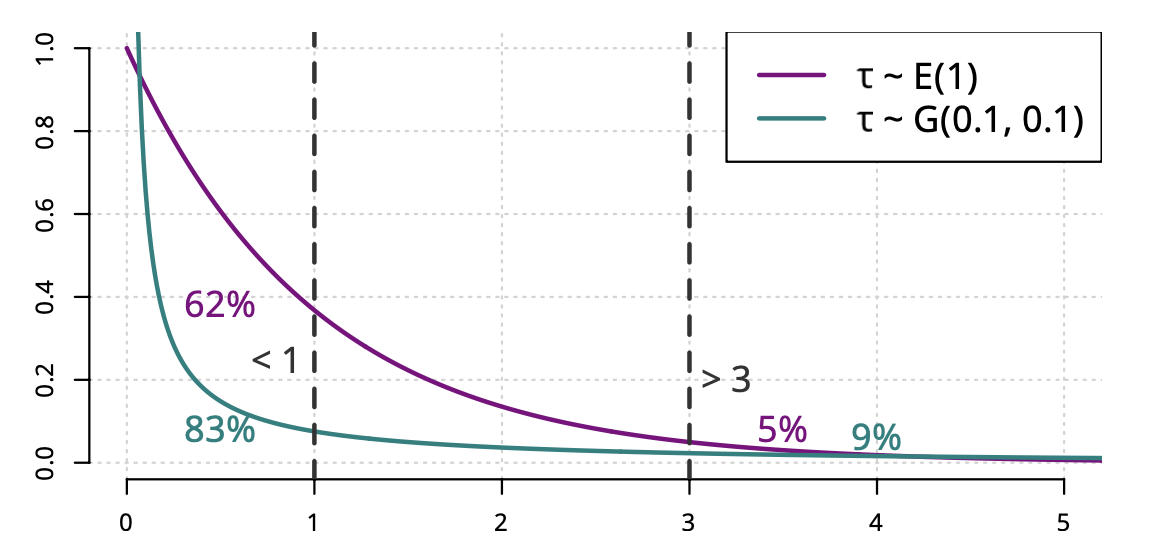
\includegraphics[width = 12cm]{shrinkage.png}
\end{center}

Not every scale-mixture prior induces shrinkage, such as $\beta\mid\eta\sim t_{2\eta}(0,\lambda^2)$:

\[
	\beta_j\mid\tau_j^2\sim\mathcal{N}(0,\lambda^2\tau^2_j), \qquad \tau^2_j\sim G^{-1}(\eta,\eta).
\]

\begin{center}
	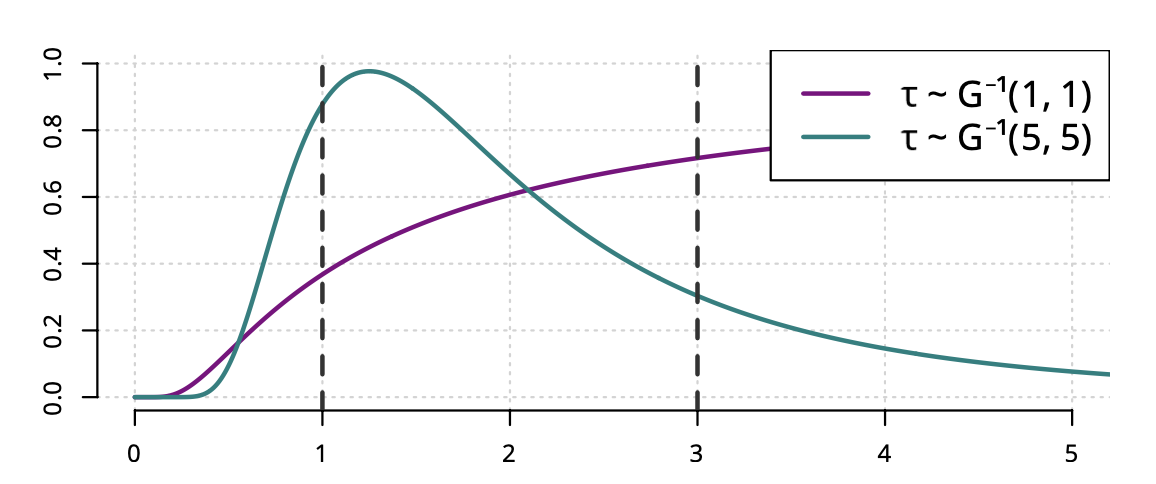
\includegraphics[width = 12cm]{noshrinkage.png}
\end{center}


% -----------------------------------------------------

\section{Bayesian Vector Autoregressions}

\subsection{Bayesian Estimation of a VAR}

A reduced-form VAR($p$) model is given by

\begin{equation}
	\bm{y}_t = \bm{c} + \bm{A}_1\bm{y}_{t-1} + \ldots + \bm{A}_p\bm{y}_{t-p} + \bm{\varepsilon}_t, \qquad \bm{\varepsilon}_t \sim \mathcal{N}_M(\bm{0},\bm{\Sigma}).
\end{equation}

More compactly, we can write it using the lag polynomial as 

\[
	\bm{A}(L)\bm{y}_t = \bm{c} + \bm{\varepsilon}_t.
\]

We can rewrite any VAR($p$) process as a VAR(1) process:

\begin{align*}
	\bm{Y}_t &= \bm{v} + \bm{AY}_{t-1} + \bm{E}_t \\
	\bm{J}'\bm{Y}_t = \bm{y}_t &= \bm{J}'(\bm{v} + \bm{AY}_{t-1} + \bm{E}_t) \\ 
	\bm{J}'\bm{Y}_t = \bm{y}_t &= \bm{c} + [\bm{A}_1 \: \bm{A}_2 \: \cdots \: \bm{A}_p]\bm{Y}_{t-1} + \bm{\varepsilon}_t,
\end{align*}

where 

\begin{align*}
& \underset{M p \times 1}{\bm{Y}_{\bm{t}}} \equiv\left[\begin{array}{c}
\bm{y}_{\bm{t}} \\
\bm{y}_{\bm{t}-\bm{1}} \\
\vdots \\
\bm{y}_{\bm{t}-\bm{p}+1}
\end{array}\right], \underset{M p \times M p}{\bm{A}} \equiv\left[\begin{array}{ccccc}
\bm{A}_{\bm{1}} & \bm{A}_{\bm{2}} & \ldots & \bm{A}_{\bm{p}-\bm{1}} & \bm{A}_{\bm{p}} \\
\bm{I}_{\bm{M}} & \bm{0}_{\bm{M}} & \ldots & \bm{0}_{\bm{M}} & \bm{0}_{\bm{M}} \\
\bm{0}_{\bm{M}} & \bm{I}_{\bm{M}} & & \bm{0}_{\bm{M}} & \bm{0}_{\bm{M}} \\
\vdots & & \ddots & \vdots & \vdots \\
\bm{0}_{\bm{M}} & \bm{0}_{\bm{M}} & \ldots & \bm{I}_{\bm{M}} & \bm{0}_{\bm{M}}
\end{array}\right] , \\
& \underset{M p \times 1}{v} \equiv\left[\begin{array}{c}
\bm{c} \\
\bm{0}_{\bm{M}} \\
\vdots \\
\bm{0}_{\bm{M}}
\end{array}\right], \quad \underset{M p \times 1}{\bm{E}_{\bm{t}}} \equiv\left[\begin{array}{c}
\varepsilon_{\bm{t}} \\
\bm{0}_{\bm{M}} \\
\vdots \\
\bm{0}_{\bm{M}}
\end{array}\right]=\bm{J} \bm{\varepsilon}_{\mathrm{t}}, \underset{M p \times M}{\bm{J}} \equiv\left[\begin{array}{c}
\bm{I}_{\bm{M}} \\
\bm{0}_{\bm{M}} \\
\vdots \\
\bm{0}_{\bm{M}}
\end{array}\right] . \\
&
\end{align*}

We can estimate this model using OLS, generalized LS, maximum likelihood, or Bayesian techniques. As mentioned before, the curse of dimensionality says that if there are $M$ equations, $M+pM^2$ parameters have to be estimated, where $M$ is the number of variables and $p$ is the lag order. The number of free parameters (elements in $\bm{c},\bm{A}_j$ and $\bm{\Sigma}$) is given by

\[
	M(Mp+1)+\frac{(M+1)M}{2}.
\]

Writing the VAR($p$) model as

\[
	\bm{y}_t = (\underbrace{[1,\bm{y}'_{t-1},\dots,\bm{y}'_{t-p}]}_{\bm{x}_t}\underbrace{[\bm{c}',\bm{A}'_1,\dots,\bm{A}_p']}_{\bm{A}})'+\bm{\varepsilon}_t,
\]

OLS gives estimates $\hat{\bm{A}} = (\bm{X}'\bm{X})^{-1}\bm{X}'\bm{Y}$ and $\hat{\bm{\Sigma}} = (\bm{Y}-\bm{XA})'(\bm{Y}-\bm{XA})/(T-Mp-1)$. These estimates are consistent and are asymptotically normally distributed with $\hat{\bm{\alpha}} = \mathrm{vec}(\bm{A})$, where $\mathrm{vec}(\bm{A})$ is the vectorization of a matrix A obtained by stacking the columns of the matrix on top of one another:

\[
	\hat{\bm{\alpha}}\overset{LLN}{\sim}\mathcal{N}(\bm{\alpha},(\bm{X}'\bm{X})^{-1}\otimes \hat{\bm{\Sigma}}).
\]

However, OLS has a small sample bias:

\begin{center}
	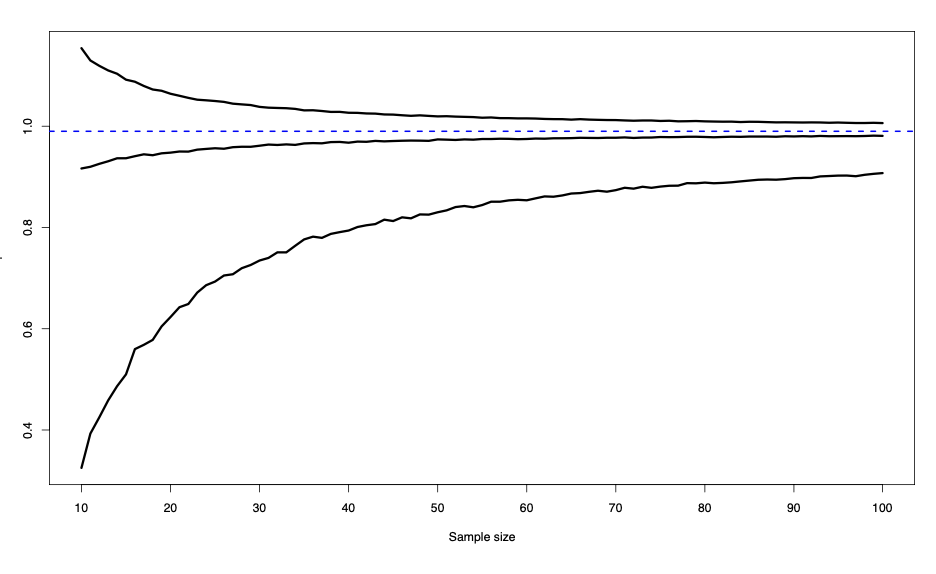
\includegraphics[width = 10cm]{smallsamplebias.png}
\end{center}

OLS has an implicit prior on lower autoregressive values. 

Bayesian methods are often used in estimating VARs. Reasons for this include proliferation of parameters (curse of dimensionality, addressed by regularization), and conditioning on initial values (via suitable prior means). To perform estimation like this, we need the likelihood of a VAR, the prior setup for the autoregressive coefficients and deterministics, and the prior setup for the variance parameters. 

\subsubsection{The Likelihood}

In the VAR model from before, 

\[
	\bm{y}_t = \bm{c} + \bm{A}_1\bm{y}_{t-1} + \ldots + \bm{A}_p\bm{y}_{t-p} + \bm{\varepsilon}_t,
\]

we can define $\bm{\alpha} = \mathrm{vec}(\bm{A}) = \mathrm{vec}((\bm{c}',\bm{A}'_1,\dots,\bm{A}_p'))$ and $\bm{x}_t = (1,\bm{y}_{t-1}', \dots, \bm{y}_{t-p}')$ and rewrite the model as

\[
	\bm{y}_t = (\bm{I}_M\otimes \bm{x}_t)\bm{\alpha}+\bm{\varepsilon}_t.
\]

The conditional likelihood is then given by

\begin{equation}
	p(\bm{y}_t\mid\bm{y}_{t-1},\dots,\bm{y}_{t-p},\bm{A},\bm{\Sigma})\sim\mathcal{N}_M([\bm{x}_t\bm{A}]',\bm{\Sigma}),
\end{equation}

or

\[
	p(\bm{y}_t\mid\bm{y}_{t-1},\dots,\bm{y}_{t-p},\bm{A},\bm{\Sigma})\sim\mathcal{N}_M((\bm{I}_M\otimes \bm{x}_t)\bm{\alpha},\bm{\Sigma}).
\]

\subsubsection{The Prior}

As prior for $\bm{A}$ (or $\bm{\alpha} = \mathrm{vec}(\bm{A})$), we can use

\begin{equation}
	p(\bm{\alpha})\sim\mathcal{N}(\underline{\bm{\alpha}},\underline{\bm{V}}).
\end{equation}

As prior for $\bm{\Sigma}$, we can use an Inverse Wishart distribution, which is something like a multivariate version of the inverse Gamma distribution. Together, this forms an independent NiW prior for our VAR.

If the sample size is small, two problems arise in estimation of a VAR: the number of parameters, and the tendency to underestimate persistence since the VAR is analyzed with the conditional likelihood. Unrestricted VARs often forecast worse than univariate random walk models. 

As prior mean, we propose

\begin{equation}
	\underline{\bm{A}} = \E{\bm{A}} = (\bm{I}_M,\bm{0},\bm{0}).
\end{equation}

That is, we set the coefficient associated with the first lag to unity, and all other coefficients to zero (which we call regularization). This induces high persistence and pushes the system towards random walk behavior.

As prior for the variance, we can use the Minnesota prior given by

\begin{equation}
	\underline{\bm{V}} = \Var{\bm{\alpha}} =
	\begin{cases}
		\left(\frac{\lambda_1}{k}\right)^2 & \text{ for $i = j$ and the $k$-th lag}, \\
		\left(\frac{\sigma^2_i}{\sigma^2_j}\right)\left(\frac{\lambda_1\lambda_2}{k}\right)^2 & \text{ for $ i \neq j $ and the $k$-th lag}, \\
		\lambda_3\sigma^2_i & \text{ for the deterministic part of the model}.
	\end{cases}
\end{equation}

This allows us to provide more shrinkage to more distant lags. The hyperparameter $\lambda_1$ governs shrinkage for own lags, $\lambda_2$ governs shrinkage for cross-variable lags, and $\lambda_3$ governs shrinkage of deterministics, and $\sigma^2_i$ is the standard deviation of an autoregressive model of variable $i$ to account for different scalings.

For the variance $\bm{\Sigma}$, we choose an Inverse Wishart prior, which is similar to a multivariate form of the Inverse Gamma distribution:

\begin{equation}
	\bm{\Sigma}\mid\bm{Y}\sim iW(\underline{s},\underline{\bm{S}}),
\end{equation}

where $\underline{s}$ are the prior degrees of freedom and $\underline{\bm{S}}$ is the prior scaling matrix. We can, for example, set the following hyperparameter values:

\begin{align*}
	\underline{s} &= M + 2, \\
	\underline{\bm{S}} &= (\underline{s}-M-1)\mathrm{diag}(\sigma_1^2,\dots,\sigma_M^2).
\end{align*}

We can also use the LDL decomposition of $\bm{\Sigma}$, 

\[
	\bm{\Sigma} = \bm{LDL}',
\]

where $\bm{L}$ is a lower triangular matrix and $\bm{D}$ is a diagonal matrix. On the off-diagonal elements of $\bm{L}$, we place Gaussian priors and on the diagonal elements of $\bm{D}$, we place inverse Gamma priors. The posterior is then very similar to the Inverse Wishart setup, but allows in contrast to the latter for equation-by-equation estimation of the autoregressive coefficients. It is also straightforward to account for heteroskedastic errors, e.g., through stochastic volatility. 

\subsubsection{The Posterior}

We then receive the following posterior for the autoregressive parameter:

\begin{equation}
	\bm{\alpha}\mid\bm{\Sigma},\bm{Y}\sim \mathcal{N}(\overline{\bm{a}},\overline{\bm{V}}),
\end{equation}

where

\begin{align*}
	\overline{\bm{V}} &= (\bm{\Sigma}^{-1}\otimes \bm{X}'\bm{X}+\underline{\bm{V}}^{-1})^{-1}, \\
	\overline{\bm{a}} &= \overline{\bm{V}}(\underline{\bm{V}}^{-1}\underline{\bm{a}}+(\bm{\Sigma}^{-1}\otimes \bm{X}')\bm{y}).
\end{align*}

The posterior for the variance is:

\begin{equation}
	\bm{\Sigma}\mid\bm{Y}\sim iW(\overline{s},\overline{\bm{S}}),
\end{equation}

where 

\begin{align*}
	\overline{s} &= T + \underline{s}, \\
	\overline{\bm{S}} &= (\bm{Y}- \bm{XA})'(\bm{Y}-\bm{XA}) + \underline{\bm{S}}.
\end{align*}

% -----------------------------------------------------

\section{Identification of Vector Autoregressions}

% -----------------------------------------------------

\subsection{Identification in Macroeconomics}

Before, we looked at tools that can be used with a VAR in its structural form, like structural impulse responses, forecast error variance, or historical decompositions. For this, we needed the structural form of a VAR($p$) model, given by

\[
\underbrace{\bm{B}_0^{-1} \bm{B}_0}_{\bm{I}} \bm{y}_t=\underbrace{\bm{B}_0^{-1} \bm{B}_1}_{\bm{A}_1} \bm{y}_{t-1}+\ldots+\underbrace{\bm{B}_0^{-1} \bm{B}_p}_{\bm{A}_p} \bm{y}_{t-p}+\overbrace{\bm{B}_0^{-1} \bm{e}_t}^{\varepsilon_t}, \quad \bm{e}_t \sim \mathcal{N}\left(0, \bm{I}_{\bm{M}}\right)
\]

Before, we assumed $\bm{B}_0^{-1}$ to be known. In this section, we will investigate how to find $\bm{B}_0^{-1}$, that is, how to identify a VAR.

Identification means to draw causal or structural conclusions from the correlations we observe in the data. In macroeconomics, this is difficult, since we need to find exogenous variation in the shock we would like to analyze. Experiments in macroeconomics are generally not possible, and even quasi-experiments are very difficult, since macroeconomic policies tend to hit the entire economy and not one separable part of it.

The reduced form of a VAR model (for simplicity a VAR(1) model is shown) is given by

\begin{equation}
	\bm{y}_t = \bm{A}_1\bm{y}_{t-1}+\bm{\varepsilon}_t,\qquad \bm{\varepsilon}_t = \bm{B}_0^{-1}\bm{e}_t\sim\mathcal{N}(\bm{0},\bm{\Sigma}_\varepsilon),
\end{equation}

and the structural form is given by

\begin{equation}
	\bm{B}_0\bm{y}_t = \bm{B}_1\bm{y}_{t-1}+\bm{e}_t, \qquad \bm{A}_1 = \bm{B}_0^{-1}\bm{B}_1.
\end{equation}

In the reduced form, the number of free parameters is 

\[
	\underbrace{M^2}_{\text{in }\bm{A}_1} + \underbrace{\frac{M\times (M+1)}{2}}_{\text{in $\bm{\Sigma}_\varepsilon$ (symmetric)}},
\]

and in the structural form, it is

\[
	\underbrace{M^2}_{\text{in }\bm{B}_0} + \underbrace{M^2}_{\text{in }\bm{B}_1}. 
\]

The difference, that is, the number of restrictions we need to impose on $\bm{B}_0^{-1}$, is therefore

\[
	M^2 - \frac{M^2}{2} - \frac{M}{2} = \frac{M \times (M - 1)}{2}.
\]

\subsection{Macroeconomic Shocks}

We are interested in identifying an economically meaningful structural shock. It should be exogenous with respect to other current and lagged endogenous variables in the model, uncorrelated with other exogenous shocks (which is hard to defend), and represent either unanticipated movements in exogenous variables or news about future movements in exogenous variables. Examples in macroeconomics include monetary policy shocks, fiscal policy shocks, supply side shocks, demand side shocks, uncertainty shocks, etc. 

Consider, for example, a monetary policy shock (that should in principle be free of political influence). The monetary policy shock $e_t^{MP}$ reflects the preferences of the monetary authority and is subject to its strategic considerations and technical factors.

\subsection{Identification Schemes}

We can impose long-run restrictions, short-run restrictions and sign restrictions. Other identification strategies include narrative methods, external instruments / Proxy VARs (where we assume to have a relevant and contemporaneously exogenous instrument for a shock, which means that projecting it on the reduced form errors, which are linear functions of the structural errors, will generate a (scaled) estimate of the structural errors under the identifying assumptions), or high-frequency identification (e.g., looking only at a 30-minute window around policy announcements).

\subsubsection{Short-Run Restrictions}

We can define that a shock has no contemporaneous impact element on a certain variable. We do this by setting the corresponding elements in $\bm{B}_0^{-1}$ to zero, such that

\[
	\bm{B}_0^{-1}
	=
	\begin{bmatrix}
		b_{11} & 0 & 0 \\
		b_{21} & b_{22} & 0 \\
		b_{31} & b_{32} & b_{33}
	\end{bmatrix}
	\quad 
	\text{ or }
	\quad
	\bm{B}_0^{-1}
	=
	\begin{bmatrix}
		* & 0 & 0 \\
		* & b_{22} & b_{23} \\
		* & * & *
	\end{bmatrix}
\]

We could also impose linear restrictions on some elements of $\bm{B}_0^{-1}$ instead of setting them to zero. However, we need to argue for any identification scheme to be economically meaningful.

Consider as an example the macroeconomic model where $\bm{y}_t = [\tilde{y}_t,\pi_t,r_t]$, where the elements are output growth, inflation, and the short-term interest rate. We can estimate a reduced-form VAR(1) process

\[
	\bm{y}_t = \bm{A}_1\bm{y}_{t-1}+\bm{\varepsilon}_t, \qquad \bm{\varepsilon}_t\sim\mathcal{N}_M(\bm{0},\bm{\Sigma}). 
\]

Finding the structural form of the process, we get

\begin{align*}
	\bm{B}_0^{-1}\bm{y}_t &= \bm{B}_1\bm{y}_{t-1} + \bm{e}_t, \qquad \bm{e}_t \sim \mathcal{N}_M(\bm{0},\bm{I}_M) \\
	\bm{y}_t &= \bm{B}_0^{-1}\bm{B}_1\bm{y}_{t-1} + \bm{B}_0^{-1}\bm{e}_t \\
	\bm{y}_t &= \bm{A}_1\bm{y}_{t-1}+\bm{\varepsilon}_t.
\end{align*}

From this, we know that

\[
 \underbrace{
 \begin{bmatrix}
 	\varepsilon_t^{\tilde{y}} \\
 	\varepsilon_t^\pi \\
 	\varepsilon_t^r
 \end{bmatrix}
 }_{\bm{\varepsilon}_t}
 =
 \underbrace{
 \begin{bmatrix}
 	b_0^{11} & b_0^{12} & b_0^{13} \\
 	b_0^{21} & b_0^{22} & b_0^{23} \\
 	b_0^{31} & b_0^{32} & b_0^{33} 
 \end{bmatrix}
 }_{\bm{B}_0^{-1}}
 \underbrace{
 \begin{bmatrix}
 	e_t^{\tilde{y}} \\
 	e_t^\pi \\
 	e_t^r
 \end{bmatrix}
 }_{\bm{e}_t}
\]

This is a system of three linear equations in nine unknowns. The variance,

\[
	\bm{\Sigma}
	=
	\begin{bmatrix}
		\sigma_{11}^2 & \sigma_{12}^2 & \sigma_{13}^2 \\
		\sigma_{12}^2 & \sigma_{22}^2 & \sigma_{23}^2 \\
		\sigma_{13}^2 & \sigma_{23}^2 & \sigma_{33}^2 
	\end{bmatrix}
\]

provides six parameters, meaning that we need to impose three additional restrictions to solve the system. 

A simple choice is to set $\bm{B}_0^{-1} = \bm{P}$, where $\bm{P}$ is the lower-triangular Cholesky decomposition of $\bm{\Sigma}_\varepsilon$. This is because by construction, $\bm{\varepsilon}_t = \bm{B}_0^{-1}\bm{e}_t \Leftrightarrow \bm{e}_t = \bm{B}_0\bm{\varepsilon}_t$. Hence, the variance-covariance matrix of the reduced form errors is

\[
	\bm{\Sigma}_\varepsilon = \E{\bm{\varepsilon}_t\bm{\varepsilon}_t'} = \bm{B}_0^{-1}\E{\bm{e}_t\bm{e}_t'}\bm{B}_0^{-1\prime} = \bm{B}_0^{-1}\bm{\Sigma}_e\bm{B}_0^{-1\prime} = \bm{B}_0^{-1}\bm{B}_0^{-1\prime}.
\]

The Cholesky decomposition can in a way be understood as “taking the square root” in matrix form. By applying a Cholesky decomposition of $\bm{\Sigma}_\varepsilon$, we therefore obtain $\bm{\Sigma}_\varepsilon = \bm{PP}'$, but also $\bm{\Sigma}_\varepsilon = \bm{B}_0^{-1}\bm{B}_0^{-1\prime}$, where both $\bm{P}$ and $\bm{B}_0^{-1}$ are lower triangular. Therefore,

\[
	\bm{P} = \bm{B}_0^{-1},
\]

which means identification. 

To identify $\bm{B}_0^{-1}$, we need to impose $M(M-1)/2$ restrictions. In the case of $M=2$, the Cholesky decomposition is

\[
	\bm{P} = 
	\begin{pmatrix}
		\sqrt{\sigma_{11}} & 0 \\
		\frac{\sigma_{12}}{\sqrt{\sigma_{11}}} & \sqrt{\sigma_{22}-\frac{1}{\sigma_{11}}\sigma^2_{12}},
	\end{pmatrix}
\]

where imposing one single zero restriction yields exact identification. We have recursive ordering for instantaneous responses: $y_{1t}$ depends only on $e_{1t}$, $y_{2t}$ depends on $e_{1t}$ and $e_{2t}$. Given a certain ordering of variables, the decomposition is unique. However, it is not unique w.r.t. the ordering of the variables as there exist $M!$ possible orderings. Permuting the order of elements in $\bm{y}$ yields different orthogonal VMA representations. Therefore, the ordering of variables matters.

In the example from before, defining $\bm{B}_0^{-1} = \bm{P}$ as the lower triangular Cholesky part of $\bm{\Sigma}_\varepsilon$, we get

\[
 \begin{bmatrix}
 	\varepsilon_t^{\tilde{y}} \\
 	\varepsilon_t^\pi \\
 	\varepsilon_t^r
 \end{bmatrix}
 =
 \begin{bmatrix}
 	p^{11} & 0 & 0 \\
 	p^{21} & p^{22} & 0 \\
 	p^{31} & p^{32} & p^{33} 
 \end{bmatrix}
 \begin{bmatrix}
 	e_t^{\tilde{y}} \\
 	e_t^\pi \\
 	e_t^r
 \end{bmatrix}
 .
\]

The system is now identified. From an interpretation perspective, the restrictions imply the following three equations:

\begin{align*}
	\Delta y_t &= \dots + p_{11} e_t^{\tilde{y}_t} \\
	\pi_t &= \dots + p_{21} e_t^{\tilde{y}_t} + p_{22} e_t^{\pi_t} \\
	r_t &= \dots + p_{31} e_t^{\tilde{y}_t} + p_{32} e_t^{\pi_t} + p_{33} e_t^{r_t}
\end{align*}

We can think of the first two equations as being aggregate demand and aggregate supply equations. AD shocks then move both output and prices on impact, whereas AS shocks move prices only. This can be visualized by a horizontal AD curve and an upward-sloping AS curve. The monetary policy authority then responds systematically to innovations in prices and output, and any change not accounted by these responses marks an exogenous monetary policy shock. 

It is important to note that we assume that output and prices are not responding to interest rate shocks within a quarter/month, which may be plausible for a month, but not for a quarter.

\subsubsection{Sign Restrictions}

For short-run restrictions we set the contemporaneous reactions of variables to certain shocks to a fixed value, usually to zero, a priori. Economic theory often suggests rather how and not when variables react to shocks; not necessarily giving an exact response. Hence, an alternative approach would be to restrict reactions of variables to increase/decrease given a certain shock → sign restrictions.

Consider a simple bivariate model of a goods market with a demand shock ($e_t^{\text{demand}}$) and a supply shock ($e_t^{\text{supply}}$). As before, the relationship between the reduced-form residuals $\bm{\varepsilon}_t$ and the structural shocks is then 

\[
	\bm{\varepsilon}_t = \bm{B}_0^{-1}\bm{e}_t, 
\]

where $\bm{\varepsilon}_t = (\varepsilon_t^q,\varepsilon_t^p)$ and $\bm{e}_t = (e_t^{\text{supply}}, e_t^{\text{demand}})$. Identifying this model using short-run zero restrictions would imply, for example, production not responding contemporaneously to a price increase, meaning that the supply curve would be horizontal. This would be hard to argue for economically. 

In general, a supply shock will increase quantity and reduce the price, while a demand shock raises both of them, which tells us something about the sign of the effect. We can therefore impose

\[
	\begin{pmatrix}
		\varepsilon_t^q \\
		\varepsilon_t^p
	\end{pmatrix}
	=
	\begin{bmatrix}
		+ & + \\
		- & +
	\end{bmatrix}
	\begin{pmatrix}
		e_t^{\text{supply}} \\
		e_t^{\text{demand}}
	\end{pmatrix},
\]

where $+$ and $-$ indicate strictly positive or negative signs of the parameters in the structural multiplier matrix. In this, shocks cannot share the same sign pattern because then we could not identify them separately. Parameters of $\bm{B}_0^{-1}$ are no longer point identified, but set identified. This complicates estimation. Sign restrictions can also be combined with zero restrictions. The sign‐identified model does not nest the recursively identified model. It relaxes the exclusion restriction but does it at the cost of restricting other parameters that were unrestricted.

Consider, for example, a VAR($p$) model in its structural form,

\[
	\bm{B}_0 \bm{y}_t=\bm{B}_1 \bm{y}_{t-1}+\ldots+\bm{B}_p \bm{y}_{t-p}+\bm{e}_t, \quad \bm{e}_t \sim \mathcal{N}\left(0, \bm{I}_{\bm{M}}\right).
\]

Suppose we have our structural multiplier matrix $\bm{B}_0^{-1}$ (with $\bm{B}_0^{-1}\bm{B}_0^{-1\prime} = \bm{\Sigma}_\varepsilon$) and we can find a full matrix $\bm{Q}$ such that

\[
	\bm{\varepsilon}_t = \bm{B}_0^{-1}\bm{Q}\bm{e}_t, \qquad\text{implying that } \bm{\Sigma}_\varepsilon = \bm{B}_0^{-1} \bm{QQ}'\bm{B}_0^{-1\prime}.
\]

This holds if $\bm{Q}$ is an orthonormal rotation matrix, $\bm{QQ}' = \bm{I}_M$. We can search for $\bm{Q}$ stochastically or deterministically such that $\bm{C} = \bm{B}_0^{-1}\bm{Q}$ fulfills the sign restriction. For each value of $\bm{\Sigma}_\varepsilon$, there is a continuum of orthonormal $\bm{Q}$ that all satisfy the constrains, which means that we have set identification.

There are several algorithms to find $\bm{Q}$. The most efficient one for larger systems is based on the Householder transformation:

\begin{enumerate}
	\item Draw each element of $\tilde{\bm{S}}(M\times M)$ from $\mathcal{N}(0,1)$. 
	\item Compute the QR decomposition of $\tilde{\bm{S}}$. The $\bm{Q}$ factor is a candidate rotation.
	\item Compute $\bm{C} = \bm{B}_0^{-1}\bm{Q}$ and the associated IRFs and check whether the constraints are fulfilled. 
	\item If so, store the IRFs. If not, discard them.
	\item Perform $N$ replications and report the median impulse response along with some quantiles.
\end{enumerate}

Often, we only have knowledge about the effects of some shocks, but not others. In other cases, only one shock is of interest. In the example of above, not knowing about the effects of a supply shock on price and quantity would mean that

\[
	\begin{pmatrix}
		\varepsilon_t^q \\
		\varepsilon_t^p
	\end{pmatrix}
	=
	\begin{bmatrix}
		? & + \\
		? & +
	\end{bmatrix}
	\begin{pmatrix}
		e_t^{\text{supply}} \\
		e_t^{\text{demand}}
	\end{pmatrix},
\]

Checking only the second column of $\bm{C}$ would in this case not be enough, as a possible solution for the signs of it could be

\[
	\begin{bmatrix}
		+ & + \\
		+ & +
	\end{bmatrix},
\]

which would not allow for the distinction of the shocks. Admissible draws would be

\[
	\begin{bmatrix}
		+ & + \\
		- & +
	\end{bmatrix}
	\text{ or }
	\begin{bmatrix}
		- & + \\
		+ & +
	\end{bmatrix}.
\]

Under sign restriction based IRFs, we do not obtain unique point estimates of the impulse response function. The structural models are then only set identified. Computing classical confidence intervals in a frequentist setting is then complicated, but Bayesian methods allow for more precise and reliable confidence bounds while also incorporating parameter uncertainty. To achieve this, we can get posterior draws of the parameters $\bm{A}$ and $\bm{\Sigma}$, compute IRFS with a $\bm{Q}$, and then compute quantiles.

% -----------------------------------------------------

\end{document}